\ifx\allfiles\undefined
\documentclass[12pt, a4paper, oneside]{ctexbook}
%\usepackage{microtype}
\usepackage{amsmath, esint,amsthm, amssymb, bm, color, framed, graphicx, imakeidx, geometry,
hyperref, mathrsfs,lipsum,fancyhdr,indentfirst,array,tabularx,float,prettyref,stmaryrd}
%文内引用
%插入书签:\label{myref:引用内容(英文字母,中文出现了编译错误)}
%引用书签:\prettyref{myref:引用内容}

\allowdisplaybreaks[4]

%简化的指令
%\renewcommand{\i}{\mathrm{i}}%虚数i
\newcommand{\di }{\text{d}}%微分
\newcommand{\pian }{\partial}%偏导数
\newcommand{\die }{\textbf{d}}%外微分
\newcommand{\fuyi }{^{-1}}%逆映射
\newcommand{\card }{\text{card}}%势
\newcommand{\R }{\mathbb{R}}%实数
\newcommand{\Z }{\mathbb{Z}}%整数
\newcommand{\RR }{$\R\ $}%实数(文本)
\newcommand{\Rn }{$\R^n\ $}%实数(文本)
\newcommand{\N }{\mathbb{N}}%自然数
\renewcommand{\S}{\mathcal{S}}%S
\newcommand{\fai }{\varphi}%常用的那个小phi
\newcommand{\e }{\vec{e}}%向量e
\newcommand{\Id }{\text{Id}}%单位元
\newcommand{\continue }{\text{连续}}%连续
\newcommand{\C }{\mathcal{C}}%连续函数类
\newcommand{\Com }{\mathbb{C}}%复数
\newcommand{\M }{\mathcal{M}}%矩阵
\newcommand{\Hess }{\text{Hess}}%Hess矩阵
\newcommand{\normmm}[1]{{\left\vert\kern-0.25ex\left\vert\kern-0.25ex\left\vert #1 
   \right\vert\kern-0.25ex\right\vert\kern-0.25ex\right\vert}}%|||v|||三个竖线的范数
%常用的文本里的字母
\newcommand{\x }{$x$}\newcommand{\xo }{$x_0$}
\newcommand{\y }{$y$}\newcommand{\yo }{$y_0$}
\newcommand{\z }{$z$}\newcommand{\zo }{$z_0$}
\newcommand{\n }{$n$}\newcommand{\f  }{$ f $}

\title{
\vspace{-2cm}
  \begin{figure}[!t]%插入题目的图片
    \centering
    
\includegraphics[width=14cm]{shulijichu-2.png}
  \end{figure}
  \vspace{-2cm}
  {\Huge{\textbf{工程师学院数学理论基础\\
Fondements des Théories Mathématiques de l'Ecole d'Ingénieur de Chimie Pékin\\
第四部分:微积分理论\\
Partie IV: Calcul Differentiel et Calcul Intégral
}}}
}
\author{Augustin}
\date{最后更新于:\today}
\linespread{1.5}
\makeindex

\setcounter{tocdepth}{1}%两个2说明只显示到subsection
\setcounter{secnumdepth}{2}

%\def\allfiles{}
\begin{document}
\newrefformat{myref}{第\ref{#1} 节}
\vspace{-3cm}
\maketitle
\tableofcontents
\else
\part{微积分理论\\ Calcul Differentiel et Calcul Intégral}
\fi
%开始本部分正文
\chapter{多元函数微分学\\ Différenciation Multifonctionnelle}
  首先我需要声明一下,可能不同于其他书籍资料都是在确定的$\R^n$上讨论多元函数的微分问题,
  本章大部分内容将会略微抽象到赋范空间或者Banach空间上讨论,但其实没有有什么区别,仅仅是换了一种更“高观点”的表达方式.
  采用这种方式是因为我们已经介绍了赋范空间,把多元函数这里的内容放在了相对后面的位置.所以请不要跳过前面的内容直接学这里.
  如果看不懂赋范空间也没关系,只需要把本章所有的$\left\lVert \cdot \right\rVert _E$或者$\left\lVert \cdot \right\rVert _F$之类的都简单地理解成向量的模长也可以.
\section{可微函数 Fonction Différentiable}
  \subsection{Définition}
    设赋范空间$E$,$F$上的映射
    $$
    f:U\subset E\rightarrow F
    $$
    考虑$E$到$F$上的连续线性映射空间$\mathcal{L}(E;F)$,
    若对$x\in U$,存在$\ell\in \mathcal{L}(E;F)$,使得
    $$
      \lim_{h \to 0_E}\frac{\left\lVert f(x+h)-f(x)-\ell(h)\right\rVert _F }{\left\lVert h\right\rVert _E}  =0
    $$
    则称$f$在$x$点处是可微的(différentiable).若对于任意$x\in U$,$f$在$x$点处都是可微的,则称其为$U$上的可微函数.
    此外,记$\ell h=\di f(x)\cdot h$,称$\di f(x)$为$f$在$x$处的微分(différentielle).\\
    \indent
    La fonction $f$ est différentiable en un point $x\in U$ s'il existe $\ell\in \mathcal{L}(E; F) $ tel que 
    $\lim_{h \to 0_E}\frac{\left\lVert f(x+h)-f(x)-\ell(h)\right\rVert _F }{\left\lVert h\right\rVert _E}  =0$.


    该定义的另一种等价表述为:
    $$
    \left\lVert f(x+h)-f(x)-\ell(h)\right\rVert _F =\varepsilon(h)\left\lVert h \right\rVert _E,\,\varepsilon (h)\xrightarrow[h\rightarrow 0_E]{}0
    $$
    或者亦可以将$\varepsilon(h)\left\lVert h \right\rVert _E$写作$o \left\lVert r(h) \right\rVert _E$.
    此时$r(h)$称余项,$\ell$称线性主部(有时也记作$A$).
    \subsubsection{可微一定连续}
    $f$在$x$点处可微则$f$在$x$点处连续.由以下三角不等式即可证明.
    $$
    \left\lVert f(x+h)-f(x)\right\rVert _F\leq \varepsilon(h)\left\lVert h \right\rVert _E+\left\lVert \ell(h) \right\rVert _F
    $$
\subsection{微分 Différentielle}
    严谨地定义微分,其表示一个线性映射:
    $$
      \di f:U\rightarrow \mathcal{L}(E;F)
    $$
    $$
      x\mapsto \di f(x)
    $$
    换句话说,$\di f$和$\di f(x)$是两码事,一个是函数,一个是值.两者的连续性没有任何关系.
    \subsubsection{Proposition}
    设$f:U\subset E\rightarrow F$在$x\in U$处可微,$g:V\subset F\rightarrow G$在$f(x)\in V$处可微,则有
    $g\circ f$在$x\in U$处可微且
    $$
    \di (g\circ f)(x)=\di g(f(x))\circ \di f(x)
    $$
\subsection{连续可微 Continûment Différentiable}
    考虑函数$f:U\subseteq E\rightarrow F$在任意$x\in U$上都是可微的.对其微分:
    $$
      \di f:U\subseteq E\rightarrow \mathcal{L} (E:F)
    $$
    $$
      x\mapsto \di f(x)
    $$
    若$\di f$是连续函数,则称$f$是连续可微的(Continûment Différentiable),记为$f\in\C^1$.



\section{$\R^n$上的微分 Différentielle sur $\R^n$}
\subsection{$\R^n$上的可微函数 }
    如果赋范空间是$\R^n$,也就是大多数书上的那样,有:
    $$
      f:\R^n\rightarrow \R^m
    $$
    $$
    (x_1,x_2,\dots,x_n)\mapsto 
    \begin{pmatrix}
      f_1(x_1,x_2,\dots,x_n)\\
      f_2(x_1,x_2,\dots,x_n)\\
      \vdots\\
     f_m(x_1,x_2,\dots,x_n)
     \end{pmatrix}
    $$
    对点$x=(x_1,x_2,\dots,x_n)$,若有
    $$
    f(x+h)-f(x)=Ah+r(h),\left\lVert r(h) \right\rVert =o\left\lVert r(h) \right\rVert 
    $$
    则称$f$在点$x$处可微.$Ah$称其微分,记为$\di f$.此时又称$A$为线性主部,$r(h)$为余项.
\subsection{偏导数 Dérivées partielles}
    考虑可微函数$f:U\subset \R^n \rightarrow F$对$x=(x_1,x_2,\dots,x_n)\in U$中的任意$i\in [\![1,n]\!]$,可以构造一个$x_i$的邻域:
    $$
      V_i(x)=\{t\in\R\,|\,(x_1,\dots,x_{i-1},t,x_{i+1},\dots,x_n)\in U \}
    $$
    则定义映射application partielle
    $$
      g_i:V_i(x)\rightarrow F
    $$
    $$
      t\mapsto f(x_1,\dots,x_{i-1},t,x_{i+1},\dots,x_n)=f(x+(t-x_i)e_i)
    $$
    称映射$g_i(t)$关于$t$的导数为$f(x_1,\dots,x_i,\dots,x_n)$关于$x_i$的偏导数.
    一般采用的偏导数符号有三种:\label{myref:lagrangenote}
  \begin{align*}
    & \frac{\partial f}{\partial x_i}(x_0)\text{ 称为Leibniz符号}\\
    & f'_{x_i}(x_0)\text{ 或 }f_{x_i}(x_0) \text{ 称为Lagrange符号}\\
    & \partial_{x_i}f(x_0) \text{ 称为Euler符号}
  \end{align*}
\subsection{偏导与微分}
  $$
    \di f(x)\cdot h=\di f(x)\cdot(\sum_{i=1}^{n}h_ie_i)=\sum_{i=1}^{n}h_i\di f(x)\cdot e_i=\sum_{i=1}^{n} h_i\frac{\pian f}{\pian x_i}(x)
  $$
  设映射:
  $$
    \di x_i:\R^n\rightarrow \R
  $$
  $$
    h\mapsto h_i
  $$
  则有:
  $$
    \di f(x)=\sum_{i=1}^{n}\frac{\pian f}{\pian x_i}(x)\di x_i
  $$
  \subsubsection{Proposition}
  向量值函数$f:U\subseteq \R^d\rightarrow F\subseteq \R^p$是连续可微的,
  当且仅当其所有$p$个偏导数都存在且在$U$上是连续的.
\subsection{线性主部}
    显然对于$\forall (m,n)\in\R^2$, $A$是一个$m\times n$矩阵,其中每一项都是某个方向函数对于某个方向的向量的偏导,即:
    $$
     A=\begin{pmatrix}
      \frac{\partial f_1}{\partial x_1}&\frac{\partial f_1}{\partial x_2}  &\cdots  &\frac{\partial f_1}{\partial x_n} \\
      \frac{\partial f_2}{\partial x_1}&\frac{\partial f_2}{\partial x_2}  & \cdots & \frac{\partial f_2}{\partial x_n}\\ 
      \vdots& \vdots & \ddots  & \vdots\\
      \frac{\partial f_m}{\partial x_1}&\frac{\partial f_m}{\partial x_2} &\cdots & \frac{\partial f_m}{\partial x_n} 
    \end{pmatrix}
    $$
    为了严谨,我们应当证明这里的线性主部是唯一的.我们假设该函数有两个线性主部$A_1$和$A_2$,并设它们的差$B=A_1-A_2$.
    则有:
    $$
      \left\lVert Bh\right\rVert \leq\left\lVert f(x+h)-f(x)-A_1h\right\rVert +\left\lVert f(x+h)-f(x)-A_2h\right\rVert
    $$
    易知对于任意非0的$h$,有$\frac{\left\lVert B(th)\right\rVert}{\left\lvert th\right\rvert}\xrightarrow[t\rightarrow 0]{}0$,且由于$B$是线性的,与$t$无关,
    故$Bh=0\Rightarrow B=0\Rightarrow A_1=A_2$,线性主部是唯一的.
\subsection{Remarque: 偏导数不可看作两项相除}
    与一元函数的导数$\frac{d f}{d x}$可以看作两个微分项相除不同,多元函数的偏导不可看做除法.这是因为$\partial f$无法对于$\partial x$精确定义.
    下面举出一个例子:
    \subsubsection{Exemple}
    理想气体的状态方程又叫Clapeyron方程,表述为:
    $$
    pV=nRT
    $$
    对于固定的$1mol$气体,有
    $$
    \frac{\partial p}{\partial V}\cdot\frac{\partial V}{\partial T}\cdot\frac{\partial T}{\partial p}=-\frac{RT}{V^2}\cdot\frac{R}{p}\cdot\frac{V}{R}=-\frac{RT}{pV}=-1
    $$
\subsection{Exemple: Vandermonde 行列式}
    定义n阶 Vandermonde 行列式为:
    $$
    u=\begin{vmatrix}
      1 &1   &\cdots & 1 \\
      x_1 &x_2 & \cdots & x_n  \\
      x_1^2 &x_2^2 & \cdots & x_n^2  \\
      \vdots &\vdots & \vdots & \vdots   \\
      x_1^{n-1} & x_1^{n-1} &\cdots &x_n^{n-1} \\
      \end{vmatrix}
      =\prod _{1\leq i\leq j\leq n}(x_i-x_j)
    $$
    求证:\\
    \begin{align*}
      & \sum_{i = 1}^{n}  \frac{\partial u}{\partial x_i}=0\\
      & \sum_{i = 1}^{n}  x_i \frac{\partial u}{\partial x_i}=\frac{n(n-1)}{2}u
    \end{align*}
    \subsubsection{Démonstration.1}
    $$
    u(x_0+h)-u(x_0)=(\frac{\partial u}{\partial x_1},\cdots,\frac{\partial u}{\partial x_n})
    \begin{pmatrix}
      h_1\\
      \vdots\\
      h_n
     \end{pmatrix}+o(\left\lVert h\right\rVert )
    $$
    设 $ h=^\top(h,\cdots,h)$,则有:
    $$
    u(x)=\prod _{1\leq i\leq j\leq n}(x_i-x_j)=\prod _{1\leq i\leq j\leq n}(x_i+h-x_j-h)=u(x+h)
    $$
    即
    $$
    0=(\frac{\partial u}{\partial x_1},\cdots,\frac{\partial u}{\partial x_n})h+o(\left\lVert h\right\rVert )=\sum_{i = 1}^{n}  \frac{\partial u}{\partial x_i}+o(1)
    $$
    \subsubsection{Démonstration.2}
    设$h=^\top(x_1h,x_2h,\cdots,x_nh)$,则
    $$
    u(x+h)=\prod _{1\leq i\leq j\leq n}[(x_i+x_ih)-(x_j+x_jh)]=\prod _{1\leq i\leq j\leq n}(h+1)(x_i-x_j)
    $$
    $$
    =(h+1)^{\binom{n}{2} }\prod _{1\leq i\leq j\leq n}(x_i-x_j)=(h+1)^{\binom{n}{2} }u
    $$
    即
    $$
    [(h+1)^{\binom{n}{2} }-1]u=h\sum_{i = 1}^{n}  x_i \frac{\partial u}{\partial x_i}+0(\left\lVert h\right\rVert )\xrightarrow[h\rightarrow 0]{}{\binom{n}{2} }u
    $$
\subsection{分量函数的可微性}
    设$D\subseteq \R^n$,对向量值函数$f:D\rightarrow \R^m$,若$f$在$x$处可微,则其每个分量函数$f_1,\cdots,f_m$在$x$处同样可微.
    \subsubsection{Démonstration}
    首先我们需要回顾\prettyref{myref:normeq}中等价范数的概念,$\R^n$空间中所有范数等价的推论,以及\prettyref{myref:LPnorme}里提到的$L^P$范数的概念.我们会利用$L^\infty$范数.
    基于此,结合范数的定义,可以得到
    $$
    \max v_{i,i\in[\![1,n]\!] }\leq \left\lVert v\right\rVert 
    $$
    现在,考虑微分的定义,有
    $$
    \left\lVert f(x+h)-f(x)-Ah\right\rVert =o\left\lVert r(h) \right\rVert 
    $$
    则可推出
    $$
    \forall i \in [\![1,m]\!],\,\left\lvert f_i(x+h)-f_i(x)-A_ih \right\rvert =o\left\lVert r(h) \right\rVert
    $$
    故$f_1,\cdots,f_m$在$x$处可微.
\subsection{方向导数 Dérivée Directionnelle}
    %方向导数与连续/可导的关系,这里还有几个结论没有给.记得补充.
    对开集$D\subseteq \mathbb{R}^n$上一点$x_0$,方向向量$\textbf{u}$,有$f:D\rightarrow \R$
    若存在$l\in\R$使得:
    $$
    \lim_{t \to 0} \frac{f(x_0+t\textbf{u})-f(x_0)}{t} =l
    $$
    则称$l$为函数$f$在$x_0$处沿$\textbf{u}$的方向导数.记为$\frac{\partial f}{\partial \textbf{u}}(x_0)$.
    有些书籍中会较为严格地定义方向导数为函数在某一点沿单位长度向量的方向导数,在这样的上下文中,
    "函数在某点沿向量$\mathbf{a}$ 方向上的导数"指的是函数在这一点沿着$\mathbf{a}$对应的单位向量$\hat{\mathbf{a}}=\frac{\mathbf{a}}{\left\lVert \mathbf{a}\right\rVert }$的方向导数.
    本节中只对方向导数做基础介绍,不进行深入讨论.
    \subsubsection{Remarque}
    要求$D$是开集,这是为了让每个点都有一个包含在定义域内的领域,使得$x_0+t\textbf{u}$仍然有定义.
    \subsubsection{方向导数的化简}
    设$l$为函数$f$在$x_0$处沿$\textbf{u}$的方向导数,显然有$f$在$x_0$处沿$\textbf{-u}$的方向导数为$-l$.
    回想一下在道路连通里运用的方法,我们只需给出一个区间映射到一条道路,使得区间的两端映射到道路的两端,并证明该映射是连续映射即可.
    这里我们采用类似的形式,设$\phi(t)=f(x_0+t\textbf{u})$在$t$充分小时有定义,且
    $$
      \phi'(0)=\lim_{t \to 0} \frac{\phi(t)-\phi(0)}{t} =\lim_{t \to 0}\frac{f(x_0+t\textbf{u})-f(x_0)}{t}=\frac{\partial f}{\partial \textbf{u}}(x_0)
    $$
    于是成功将$\frac{\partial f}{\partial \textbf{u}}(x_0)$转化为$\phi'(0)$的一元函数求导问题. 
\subsection{一阶微分形式不变性}
    一阶微分形式不变性其实就是可以把某个自变量看作另一个变量的函数,非常直观.但是从重要性来说,这又是非常严谨而不可或缺的一环.
    因此我们还需证明这个trival的结论.
    $$
    u=f(x_1,x_2,\cdots,x_n) \text{ 且 }\forall x_{i,i\in [\![1,n]\!]}, x_i=(t_1,t_2,\cdots,t_m)
    $$
    若以$x$为自变量,则有:
    $$
      du=\sum_{i=1}^{n}\frac{\partial f}{\partial x_i}dx_i
    $$
    若以$t$为自变量,则有:
    $$
      du=\sum_{j=1}^{m}(\sum_{i=1}^{n}\frac{\partial f}{\partial x_i}\frac{\partial x_i}{\partial t_j})dt_j
    $$
    $$
      =\sum_{i=1}^{n}\frac{\partial f}{\partial x_i}\sum_{j=1}^{m}\frac{\partial x_i}{\partial t_j}dt_j
    $$
    考虑后面的求和部分,有:
    $$
    \sum_{j=1}^{m}\frac{\partial x_i}{\partial t_j}dt_j=dx_i
    $$
    即该式等于
    $$
    \sum_{i=1}^{n}\frac{\partial f}{\partial x_i}\sum_{j=1}^{m}\frac{\partial x_i}{\partial t_j}dt_j = \sum_{i=1}^{n}\frac{\partial f}{\partial x_i}dx_i
    $$
    该式成为多元函数的一阶微分形式不变性.至此,我们对于多元函数的求导才有了严谨性.
    \subsubsection{Exemple}
    设$f(x,y)=\arctan(\frac{x}{y})$,求$\frac{\partial f}{\partial x}$和$\frac{\partial f}{\partial x}$.\\


    $$df=d \arctan(\frac{x}{y})=\frac{1}{1+(\frac{x}{y})^2}d(\frac{x}{y})=\frac{ydx-xdy}{x^2+y^2}=\frac{y}{x^2+y^2}dx+\frac{x}{x^2+y^2}dy$$
    又
    $$df=\frac{\partial f}{\partial x}dx+ \frac{\partial f}{\partial y}dy$$
    则可求出偏导.
\section{关于连续性的讨论 Discussion sur la continuité}

在本节里,我们会专门讨论一阶连续性的问题(主要是一阶连续).
多元函数的连续性与之前学过的一元函数的连续性不同,很多时候并不那么直观,而是需要一定的数学理解能力辅助判断.

\subsection{Remarque}
  作为总结,我们可以给出这样的示意图:
  $$
  \text{偏导数连续}\Rightarrow\text{函数可微}\Rightarrow
  \begin{cases}
    \text{函数连续} & \\
    \text{偏导存在} & \\
    \text{方向导数存在}
    \end{cases}
  $$

\section{Jacobi矩阵 Matrice Jacobienne}
    \subsection{Définition}
    考虑到前文提到的线性主部
    $$
     A=\begin{pmatrix}
      \frac{\partial f_1}{\partial x_1}&\frac{\partial f_1}{\partial x_2}  &\cdots  &\frac{\partial f_1}{\partial x_n} \\
      \frac{\partial f_2}{\partial x_1}&\frac{\partial f_2}{\partial x_2}  & \cdots & \frac{\partial f_2}{\partial x_n}\\ 
      \vdots& \vdots & \ddots  & \vdots\\
      \frac{\partial f_m}{\partial x_1}&\frac{\partial f_m}{\partial x_2} &\cdots & \frac{\partial f_m}{\partial x_n} 
     \end{pmatrix}
    $$
    称其为Jacobi矩阵,或Jacobi算子,记作$J$.
    若$J\in\mathcal{M}_n(\R) $,则称$\det(J)$为Jacobi行列式,记作$\det(J)=\frac{\partial(f_1,f_2,\cdots,f_n)}{\partial(x_1,x_2,\cdots,x_n)}$
    \subsubsection{Remarque}
    另有一些教材将Matrice Jacobienne记为$D$(特别是在与物理相关的内容中!):
    $$
     (Df(x))_{i,j}=\frac{\partial f_i(x)}{\partial x_j}
    $$
    \subsection{线性映射的微分}
    $f:\R^n\rightarrow \R^m$,若有$f(x)=Ax$,则$A=J_f$.
    \subsubsection{Démonstration}
    设单位向量$h$
    $$
      \lim_{t \to 0}\frac{\left\lVert f(x+th)-f(x)-A(th) \right\rVert }{t}  =\lim_{t \to 0}\frac{\left\lVert A(x+th)-A(x)-A(th) \right\rVert }{t} =0 
    $$
    \subsection{Jacobi算子的运算法则}
    Jacobi算子满足以下运算法则:
    对$f,g:D\rightarrow \R^m, D\subseteq\R^n,A\in\mathcal{M}_{p\times m}(\R)$,有:
    \begin{itemize}
      \item $J(Af)=AJf$
      \item $J(f+g)=Jf+Jg$
      \item $J(^\top f\cdot g)=^\top g\cdot Jf+^\top f\cdot Jg$
    \end{itemize}
\section{$\nabla$ 算子 Opérateur $\ll$ nabla $\gg$ }%符号输入问题$\nabla$ 算子 Opérateur $\ll$ nabla $\gg$ 无法识别,怎么回事
    %大家好啊,我是说$\nearrow $的$\nearrow $物$\searrow $理$\rightsquigarrow $,今天给大家来点想看的东西.
    将Jacobi算子转置,我们就得到了另一个算子$\nabla$(nabla).这个算子经常出现在各种与物理有关的地方.

  \subsection{梯度 Gradient}
    设标量值函数(标量场)$\varphi:U\subseteq \R^p \rightarrow \R$,
    其梯度是一个$p$维矢量函数(矢量场),记为$\nabla \varphi$或者$\overrightarrow{grad} (\varphi)$, $\text{grad } \varphi$:
    $$
    \nabla \varphi=
    \begin{pmatrix}
      \frac{\partial \varphi(x)}{\partial x_1}\\
      \frac{\partial \varphi(x)}{\partial x_2}\\
      \vdots \\
      \frac{\partial \varphi(x)}{\partial x_p}
    \end{pmatrix}
    $$

    物理意义上,标量场中某一点的梯度指向这一点上标量场增长最快的方向.
    \subsubsection{Exemple}
    考虑一阶连续的标量场:\\


    三维直角坐标系中$\phi(x,y,z)$的梯度为:
    $$
    \overrightarrow{grad} (\phi)=\nabla \phi=\frac{\partial \phi}{\partial x}\overrightarrow{e_x}+\frac{\partial \phi}{\partial y}\overrightarrow{e_y}+\frac{\partial \phi}{\partial z}\overrightarrow{e_z}
    $$

    柱坐标系中$\phi(r,\varphi ,z)$的梯度为:
    $$
    \overrightarrow{grad} (\phi)=\nabla \phi=\frac{\partial \phi}{\partial r}\overrightarrow{e_r}+\frac{1}{r}\frac{\partial \phi}{\partial \varphi}\overrightarrow{e_\varphi}+\frac{\partial \phi}{\partial z}\overrightarrow{e_z}
    $$

    球坐标系中$\phi(r,\theta,\varphi)$的梯度为:
    $$
      \overrightarrow{grad} (\phi)=\nabla \phi=\frac{\partial \phi}{\partial r}\overrightarrow{e_r}+\frac{1}{r}\frac{\partial \phi}{\partial \theta}\overrightarrow{e_\theta}+\frac{1}{r\sin\theta}\frac{\partial \phi}{\partial \varphi}\overrightarrow{e_\varphi}
    $$
    \subsubsection{Remarque}
    给定一个标量场$\varphi$,其在空间内一点的梯度只取决于该点的位置,而不取决于空间的基.
  \subsection{散度 Divergence}
    设向量值函数(矢量场)$f:U\subseteq \R^p \rightarrow \R^p$,
    其散度是一个$\R$上的标量,记为$\nabla \cdot f$或$\text{div }f$:
    $$
      \nabla \cdot f=\text{tr}(Df(x))=\sum_{i=1}^{p}\frac{\partial f_i(x)}{\partial x_i}
    $$

    物理意义上,散度用于描述场中一点的有源性,散度大于0说明该点有新的通量产生,小于0说明有通量汇聚湮灭,等于零说明无源.
    例如不可压缩流体散度为0,说明流体内的粒子不会凭空产生或消失.
    \subsubsection{Exemple}
    考虑一阶连续的矢量场:\\


    三维直角坐标系中$\textbf{A}(x,y,z)=P(x,y,z)\vec{e}_x+Q(x,y,z)\vec{e}_y+R(x,y,z)\vec{e}_z$的散度为:
    $$
      \text{div } \textbf{A}=\nabla \cdot \textbf{A}=\frac{\partial P}{\partial x}+\frac{\partial Q}{\partial y}+\frac{\partial R}{\partial z}
    $$

    柱坐标系中$\textbf{A}(r,\varphi ,z)=A_r(r,\varphi ,z)\vec{e}_r+A_\varphi(r,\varphi ,z)\vec{e}_\varphi+A_z(r,\varphi ,z)\vec{e}_z$的散度为:
    $$
      \text{div } \textbf{A}=\nabla \cdot \textbf{A}=\frac{1}{r}\frac{\partial rA_r}{\partial r}+\frac{1}{r}\frac{\partial A_\varphi}{\partial \varphi}+\frac{\partial A_z}{\partial z}
    $$

    球坐标系中$\textbf{A}(r,\theta ,\varphi)=A_r(r,\theta ,\varphi)\vec{e}_r+A_\theta(r,\theta ,\varphi)\vec{e}_\theta+A_\varphi(r,\theta ,\varphi)\vec{e}_\varphi$的散度为:
    $$
      \text{div } \textbf{A}=\nabla \cdot \textbf{A}=\frac{1}{r^2}\frac{\partial r^2A_r}{\partial r}+\frac{1}{r\sin \theta}\frac{\partial\sin\theta A_\theta}{\partial \theta}+\frac{1}{r\sin\theta}\frac{\partial A_\varphi}{\partial\varphi}
    $$
  \subsection{旋度 Rotationnel}
    设三维向量值函数(矢量场)$f:U\subseteq \R^3 \rightarrow \R^3$,
    其旋度是一个3维矢量函数(矢量场),记为$\nabla\times f$或者$\overrightarrow{rot}f$, $\text{rot} f$:
    $$
    \overrightarrow{rot} (f)=\nabla\times f
    $$

    物理意义上,旋度表示在三维欧几里德空间中的向量场的无穷小量旋转.在向量场每个点上,点的旋度表示为一个向量,称为旋度向量.这个向量的特性(长度和方向)刻画了在这个点上的旋转.
    不同于梯度和散度,旋度不能简单的推广到其他维度.某些推广是可能的,但是只有在三维中,在几何上定义的向量场旋度还是向量场.
    这个现象类似于三维叉积,这个联系反应在旋度的符号上.\\

    旋度的方向是旋转的轴,它由右手定则来确定,而旋度的大小是旋转的量.
    如果向量场表示一个移动的流形的流速,则旋度是这个流形的环量面密度.
    \subsubsection{Exemple}
    考虑一阶连续的三维矢量场:\\

    直角坐标系中$\textbf{A}(x,y,z)=A_x(x,y,z)\vec{e}_x+A_y(x,y,z)\vec{e}_y+A_z(x,y,z)\vec{e}_z$的旋度为:
    $$
    \overrightarrow{rot} (f)=\nabla\times f=(\frac{\partial A_z}{\partial y}-\frac{\partial A_y}{\partial z})\vec{e}_x+
    (\frac{\partial A_x}{\partial z}-\frac{\partial A_z}{\partial x})\vec{e}_y+(\frac{\partial A_y}{\partial x}-\frac{\partial A_x}{\partial y})\vec{e}_z
    $$
    或表示为:
    $$
    \overrightarrow{rot} (\textbf{A})=\nabla\times \textbf{A}=
    \begin{vmatrix}
      \vec{e}_x&\vec{e}_y  &\vec{e}_z \\
      \frac{\partial }{\partial x}& \frac{\partial }{\partial y} &\frac{\partial }{\partial z} \\
      A_x& A_y &A_z
    \end{vmatrix}
    $$

    这里的行列式记号只有形式上的意义,因为真正的行列式中的系数应该是数值而不是向量.这种表示方法只是便于记忆旋度在直角坐标系中的表达式.
    法语内容中不常见这种行列式的形式(因为这并不严谨,行列式不能算出个向量来),但许多中文资料却以此作为帮助记忆的方式.这确实比上面的长式子更方便,因此我推荐使用这种记忆方法.\\


    柱坐标系中$\textbf{A}(r,\varphi ,z)=A_r(r,\varphi ,z)\vec{e}_r+A_\varphi(r,\varphi ,z)\vec{e}_\varphi+A_z(r,\varphi ,z)\vec{e}_z$的散度为:
    $$
    \overrightarrow{rot} (\textbf{A})=\nabla\times \textbf{A}=(\frac{1}{r}\frac{\partial A_z}{\partial \varphi}-\frac{\partial A_\varphi}{\partial z})\vec{e}_r+
    (\frac{\partial A_r}{\partial z}-\frac{\partial A_z}{\partial r})\vec{e}_\varphi+\frac{1}{r}(\frac{\partial rA_\varphi}{\partial r}-\frac{\partial A_r}{\partial \varphi})\vec{e}_z
    $$
    或表示为:
    $$
    \overrightarrow{rot} (\textbf{A})=\nabla\times \textbf{A}=
    \begin{vmatrix}
      \frac{1}{r} \vec{e}_r&\vec{e}_\varphi  &\frac{1}{r}\vec{e}_z \\
      \frac{\partial }{\partial r}& \frac{\partial }{\partial \varphi} &\frac{\partial }{\partial z} \\
      A_r& rA_\varphi &A_z
    \end{vmatrix}
    $$
    要注意的是,以上的行列式中元素并不是可交换的.实际计算时,展开式其中的每一项应该是第一行的元素乘以第二行的元素再作用于第三行的元素.\\


    球坐标系中$\textbf{A}(r,\theta ,\varphi)=A_r(r,\theta ,\varphi)\vec{e}_r+A_\theta(r,\theta ,\varphi)\vec{e}_\theta+A_\varphi(r,\theta ,\varphi)\vec{e}_\varphi$的旋度为:
    $$
    \overrightarrow{rot} (\textbf{A})=
      \frac{1}{r\sin\theta}(\frac{\partial A_\varphi \sin\theta}{\partial \theta}-\frac{\partial A_\theta}{\partial \varphi})\vec{e}_r+
      \frac{1}{r}(\frac{1}{\sin\theta}\frac{\partial A_r}{\partial \varphi}-\frac{\partial A_\varphi}{\partial r})\vec{e}_\theta+\frac{1}{r}(\frac{\partial rA_\theta}{\partial r}-\frac{\partial A_r}{\partial \theta})\vec{e}_\varphi 
    $$
    或表示为:
    $$
    \overrightarrow{rot} (\textbf{A})=\nabla\times \textbf{A}=
    \frac{1}{r^2\sin\theta} 
    \begin{vmatrix}
      \vec{e}_r&r\vec{e}_\theta  &r\sin\theta\vec{e}_\varphi \\
      \frac{\partial }{\partial r}& \frac{\partial }{ \partial \theta} &\frac{\partial }{\partial \varphi} \\
      A_r& rA_\theta &r\sin\theta A_\varphi
    \end{vmatrix}
    $$
    同样行列式不可交换元素.
    \subsection{Laplace算子 Opérateur Laplacien}
    Laplace算子是梯度和散度的复合算子,定义为$\Delta f=\nabla^2 f=\nabla\cdot(\nabla f)=\text{div }(\overrightarrow{grad} (\varphi))$.
    其物理意义在于刻画了空间的"均匀度".
    鉴于我们还没有学习高阶偏导数,这里并不打算详细将清楚Laplace算子.我们后续会补充说明它的.\\

    对三维直角坐标系中的标量值函数$f(x,y,z)$:
    $$
    \Delta f=\nabla^{2}f=\frac{\partial^{2}f}{\partial x^{2}}+\frac{\partial^{2}f}{\partial y^{2}}+\frac{\partial^{2}f}{\partial z^{2}}
    $$\\

    柱坐标系$f(r,\varphi,z)$:
    $$
    \Delta f=\frac{1}{r} \frac{\partial}{\partial r}\left(r \frac{\partial f}{\partial r}\right)+\frac{1}{r^{2}} \frac{\partial^{2} f}{\partial \theta^{2}}+\frac{\partial^{2} f}{\partial z^{2}}
    $$\\

    球坐标系$f(r,\theta,\varphi)$:
    $$
      \Delta f=\frac{1}{r^2} \frac{\partial}{\partial r}\left(r^2 \frac{\partial f}{\partial r}\right)
      +\frac{1}{r^2\sin\theta}\frac{\partial}{\partial\theta}(\sin\theta\frac{\partial f}{\partial\theta})
      +\frac{1}{r^2\sin^2\theta}\frac{\partial^2f}{\partial\varphi^2}
    $$\\

    对向量值函数,其Laplace算子为每个分量的Laplace算子组成的向量,即:
    $$
    \Delta \textbf{A}=
    \begin{pmatrix}
      \Delta A_{x_1}\\
      \Delta A_{x_2}\\
      \vdots \\
      \Delta A_{x_p}
    \end{pmatrix}
    $$\\

    或
    $$
    \Delta \textbf{A}=\nabla(\nabla\cdot\textbf{A})-\nabla\times(\nabla\times\textbf{A})
    $$

    现在我们总结一下$\nabla$算子的各种表达如下:
    \begin{figure}[!h]
      \centering
      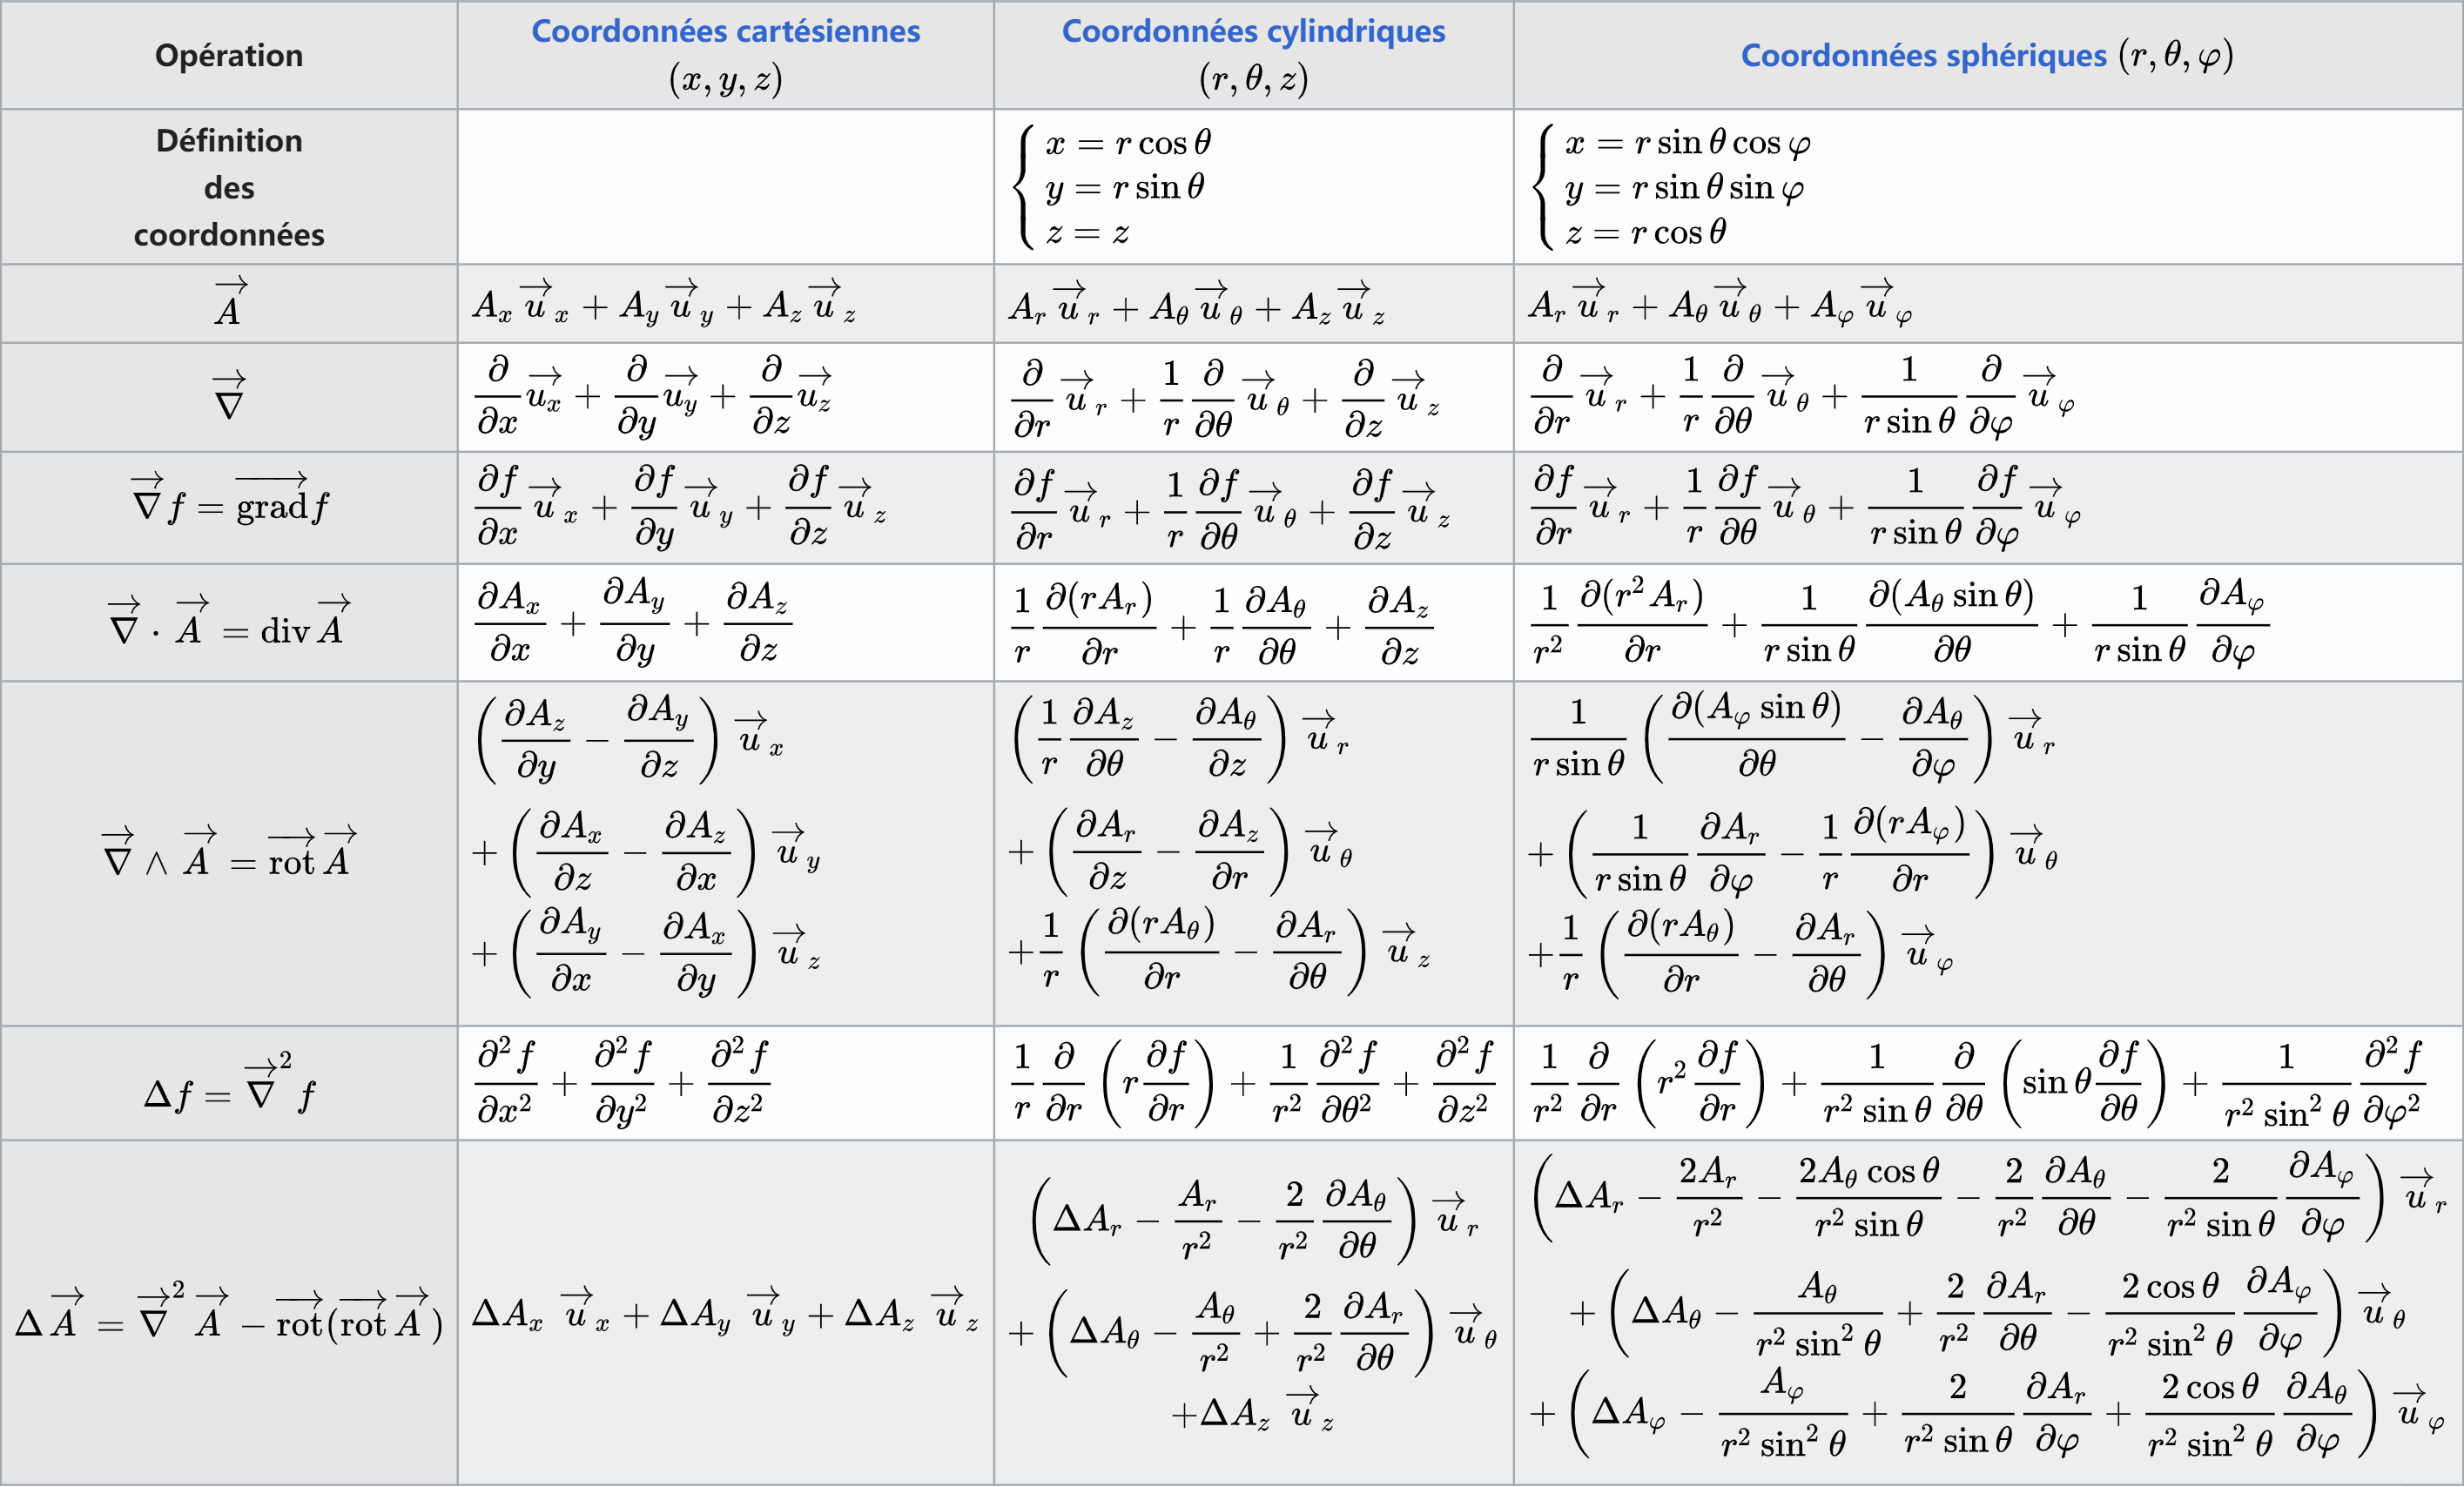
\includegraphics[scale=0.4]{nabla.png}
      \caption{$\nabla$算子(图源自法语wiki)}
      \label{fig:nabla}
    \end{figure}
  \subsection{Gauss散度定理 Théorème de flux-divergence}
    Gauss 散度定理,法语称 Théorème de flux-divergence 或者 Théorème de Green-Ostrogradski\footnote{在物理中偶尔会称Théorème de Gauss}.其说明矢量场穿过曲面的通量等于散度在曲面围起来的体积上的积分,即净流出量等于所有源点的和减去所有汇点的和.
    其在一维情况下等价于微积分基本定理,二维情况下等价于Green公式.
    $$
      \iiint \limits_{V} \text{div } \vec{F}\,dV=\oiint\limits_{\partial V}\vec{F} d\vec{S}  
    $$

\section{有限增长定理 Théorème des Accroissements Finis}
\subsection{Remarque: Rolle定理}
  设$\fai: I\subset \R\rightarrow \R$
  现在,我们将把Rolle定理推广.
\subsection{单实变函数的推广 Cas d'une variable réelle}
  设可微函数$f:I\subseteq \R\Rightarrow F$,其中$I$是开区间,$F$是实赋范向量空间.
  若有:
  $$
  \forall t\in I,\,\exists k>0,\, \left\lVert f'(t)\right\rVert _F\leq k 
  $$
  则有:
  $$
  \forall(x,y)\in I\times I,\,\left\lVert f(x)-f(y)\right\rVert _F\leq k\left\lvert x-y\right\rvert 
  $$
  \subsubsection{Démonstration}
  设$x<y$.考虑一个中间值$t\in[x,y]$.
  $$
  \forall \epsilon>0,\,\left\lVert f(x)-f(y)\right\rVert _F\leq (k+\epsilon)(t-x)+\epsilon
  $$
  通过证明以上的中间结论,加以$t$趋近于$y$即可证明推广公式.
  下面我们尝试证明这个中间结论.考虑集合:
  $$
  \mathcal{O}=\{t\in[x,y]\,|\,\left\lVert f(x)-f(y)\right\rVert _F> (k+\epsilon)(t-x)+\epsilon \}
  $$
  则$\mathcal{O}$是一个开集.下面要证明它是空集.
  利用反证法设其非空,则有下界$\underline{o}$.
  此下界$\underline{o}>x$且$\underline{o}\notin\mathcal{O}$,故有:
  $$
  \left\lVert f(\underline{o})-f(x)\right\rVert _F\leq (k+\epsilon)(\underline{o}-x)+\epsilon
  $$
  在$\underline{o}$附近,$  \exists \eta >0 ,\,\forall t\in(\underline{o},\underline{o}+\eta]$,有
  $$
    k\ge \left\lVert f'(\underline{o})\right\rVert _F\ge\frac{\left\lVert f(t)-f(\underline{o})\right\rVert _F}{\left\lvert t-\underline{o} \right\rvert} -\epsilon
  $$
  故有:
  $$
    \left\lVert f(t)-f(\underline{o})\right\rVert _F\leq (k+\epsilon)(t-\underline{o})
  $$
  可由三角不等式推出
  $$
    \left\lVert f(t)-f(\underline{o})\right\rVert _F\leq (k+\epsilon)(t-x)+\epsilon
  $$
  这说明$[\underline{o},\underline{o}+\eta]\cap\mathcal{O}=\varnothing$.
  又因为$t<y$,故对于一个足够小的$\eta$,仍有$\underline{o}+\eta<y $,
  即说明在$\underline{o} $与$\sup \mathcal{O}$中间存在至少一个$\underline{o}+\eta$,也即$\underline{o}\neq \sup \mathcal{O}$,与原假设矛盾.

\subsubsection{Proposition}
  设可微函数$f:I\subseteq \R\rightarrow F$,其中$I$是开区间,$F$是实Banach空间.
  若存在可导函数$\fai: I\rightarrow \R$使得:
  $$
  \forall t\in I,\,\exists k>0,\, \left\lVert f'(t)\right\rVert _F\leq \fai'(t)
  $$
  则有
  $$
  \forall(x,y)\in I\times I,\,\left\lVert f(x)-f(y)\right\rVert _F\leq \left\lvert \fai(x)-\fai(y)\right\rvert 
  $$
  \subsection{更一般的推广 Cas général}
  如上文所述,给出一般的赋范空间$E,F$上的可微函数函数$f:U\subseteq E\rightarrow F$.
  若有:
  $$
  \forall u\in U,\,\exists k>0,\,\normmm{\di f(u)}\leq k 
  $$
  则有:
  $$
  \forall(x,y)\in U\times U,\,\left\lVert f(x)-f(y)\right\rVert _F\leq k\left\lVert x-y\right\rVert _E
  $$
  \subsubsection{Démonstration}\noindent
  借助一个可导的辅助函数:
  $$
    g:[0,1]\rightarrow F
  $$
  $$
    t\mapsto f(x+t(y-x))
  $$
  其导数$g'(t)=\di f(x+t(y-x))(y-x)$满足:
  $$
  \forall t\in[0,1],\,\left\lVert g'(t)\right\rVert _F\leq k\left\lVert y-x\right\rVert _E
  $$
  根据单实变函数的结论,有:
  $$
  \left\lVert f(y)-f(x)\right\rVert _F=\left\lVert g(1)-g(0)\right\rVert _F\leq k\left\lVert x-y\right\rVert _E
  $$
  \subsubsection{Proposition}
  该不等式的另一种表述形式为:
  $$
  \left\lVert f(y)-f(x)\right\rVert _F\leq \sup_{t\in[0,1]}\normmm{\di f(x+t(y-x))}\left\lVert x-y\right\rVert _E
  $$
  \subsection{Proposition: sur les ouverts connexes}
    \subsubsection{Remarque: 连通子集 sous-ensemble connexe}
    考虑一个Banach空间的子空间拓扑,若除了空集和它本身之外没有既开又闭的子集,那么它就是连通的.\\
    \indent
    Un sous-ensemble d'un espace de Banach est connexe s'il n'admet pas de sous-ensemble à la fois ouvert et fermé autre que l'ensemble vide et lui-même.
    \subsubsection{Théorème}
    设连通集$U\subseteq E\rightarrow F$上的可微函数$f$,若有:
    $$
      \forall x\in U,\,\di f(x)\equiv 0
    $$
    则$f$是一个常值映射.
    \subsubsection{Démonstration}
    $\forall x\in U,\,\exists \text{ 开球}B(x,r)\subset U$.
    由有限增量定理知,$\di f=0$意味着$\forall y\in B(x,r),\,f(x)=f(y)$,故$f$在$x$附近是常值映射.
    接下来考虑逆映射$f\fuyi$.显然有$f\fuyi(\{f(x)\})\subset U\neq\varnothing$.
    又因为$\{f(x)\}$作为单点集是闭集,故$f\fuyi(\{f(x)\})$也是闭集.
    而我们前面任选的开球都是开集,因此$f\fuyi(\{f(x)\})$是$U$上非空的既开又闭的集合,只能是$U$本身.

 \subsection{Proposition: sur $\C^1$ }
  设一族有限个赋范空间$E_1,\dots,E_n$, $E=E_1\times \cdots \times E_n$
  上的可微函数:
  $$
    f:U\subseteq E \rightarrow
  $$
  $$
    x=(x_1,\dots,x_n)\mapsto f(x)
  $$
  $f$是连续可微函数当且仅当
  $$
  \forall i\in[\![1,n]\!],\,y_i\mapsto (x_1,\dots,x_{i-1},y_i,x_{i+1},\dots,x_n)
  $$
  在$y_i=x_i$处可微,且其微分对应了$U$上的一个$\mathcal{L}(E:F)$的函数.
\section{局部反演定理/反函数定理 Théorème d'Inversion Locale}
\subsection{微分同胚 Difféomorphisme}
  设$U$和$V$分别是实Banach空间$E$和$F$上的两个开集,若其上的函数$f:U\rightarrow V$满足:
  \begin{itemize}
    \item $f$是一个双射
    \item $f\in\mathcal{C}^1(U)$,即$f$是$U$上的一阶连续可微函数
    \item $f^{-1}\in\C^1(V)$,即$f$是$V$上的一阶连续可微函数
  \end{itemize}
  则称$f$是一个从$U$到$V$的微分同胚映射,简称微分同胚(Difféomorphisme).
  \subsubsection{Remarque}
  回顾\prettyref{myref:tongpei}同胚的概念.
  \subsubsection{Exemple}
  $(-\frac{\pi}{2},\frac{\pi}{2})$上的 $\sin,\,\cos$ 函数是微分同胚.
  \subsubsection{Exemple}
  $x\mapsto x^3$不是微分同胚.
  \subsubsection{Proposition}
  若$f:U\rightarrow V$是微分同胚,则$\forall x\in U,\,\di f(x)$是$E$到$F$上的同构.且有:
  $$
    \forall y\in V,\,\di f^{-1}(y)=(\di f(f^{-1}(y)))^{-1}
  $$
  \subsubsection{Démonstration}
  设$y=f(x),\,g=f^{-1}$,则有:
  $$
    g\circ f=\Id_U \text{            且             }f\circ g=\Id_V
  $$
  由复合函数的求导法则知:
  $$
  \forall x\in U,\,\di g(y)\circ \di f(x)=\Id_E\text{            且             }\di f(x)\circ \di g(y)=\Id_F
  $$
  \subsubsection{Proposition}
  若存在$E$到$F$的微分同胚,则两个空间是同构的.若其中一个是有限维的,则另一个空间也具有相同的维度.
  \subsubsection{Proposition}
  设$f:U\rightarrow V$,且$f\in\C^1$.对$a\in U$

  \subsection{Banach不动点定理 Théorème de Banach-Picard}
    设$C$是Banach空间$E$上的闭非空闭集,存在压缩映射 $h:C\rightarrow C$,即:
    $$
      \exists k\in(0,1),\,\forall (x_1,x_2)\in C^2,\,\left\lVert h(x_1)-h(x_2)\right\rVert _E\leq k\left\lVert x_1-x_2\right\rVert _E
    $$
    则$C$中有且仅有一个映射到自身的点,即:
    $$
      \exists! \,x\in C,\,h(x)=x
    $$
    \indent
    Si $C$ est un fermé non vide d'un espace de Banach $E$ et si $h:C\rightarrow C$ est contractante, 
    il existe un unique $x\in C$ tel que $h(x) = x$.
    \subsubsection{Démonstration}
    补全\prettyref{myref:yasuoyingshe} 的压缩映射再说


  \subsection{反函数定理 Théorème d'inversion globale}
  设$E$上非空开集$U$上的连续可微映射$f:U\subset E\rightarrow F,\,f\in \C^1$,
  则\f 是一个$U$到$f(U)$上的微分同胚当且仅当\f 是一个单射且其任意一点$U$上的微分都是从$E$到$F$的同构.\\
  \indent
  Soit $f : U \rightarrow F$ une application de classe $\C^1 $ avec $U$ un ouvert non vide. 
  C'est un difféomorphisme de $U$ sur $f (U)$ si et seulement si elle est injective et sa différentielle est en tout point de $U$ un isomorphisme de $E$ sur $F$.
  \subsubsection{Démonstration}

  \subsection{$\R^n$上的反函数 Cas de $\R^n$}
  设单射$f:U\subset \R^n\rightarrow \R^n,\,f\in\C^1$,\f 是一个微分同胚当且仅当其Jacobi矩阵在$U$上不为0(可逆).\\
  \indent
  Soit $U$ un ouvert de $\R^n$ et $f : U \rightarrow \R^n$ injective et de classe $\C^1 $.
  Alors\f est un difféomorphisme si et seulement si le déterminant de sa matrice jacobienne ne s'annule pas sur $U$.

\section{隐函数定理 Théorème des Fonctions Implicites}
\subsection{隐函数 Fonction implicite}
    对非线性方程$f(x,y)=0$,若可以将$y$表示为$x$的函数,即$y=\fai(x)$,则称方程隐含(implicitement)地定义了$y$,或称$y$是$x$的隐函数.
    \subsubsection{Exemple}
\subsection{隐函数定理}
  Banach空间上的隐函数定理是反函数定理的另一种表达方式,或者说二者是等价的.
  该定理的表示为:\\

  \indent
  设Banach空间$E,\,F,\,G$ 上的函数$f:U\subset E\times F\rightarrow G,\,f\in\C^1$.
  设存在$(a,b)\in U$ 使得$f(a,b)=0_G$,且关于$y$的偏微分$\di_2f(a,b)$是$F$到$G$上的同构,
  则存在$U$中关于$(a,b)$的邻域$U_{(a,b)}$和$E$中关于$a$的邻域$W_a$,以及函数
  $\fai:W_a\rightarrow F,\,\fai\in \C^1$使得:
  $$
    ((x,y)\in U_{(a,b)}\land f(x,y)=0_G)\Leftrightarrow y=\fai(x)
  $$
  \indent
  Soit $U$ un ouvert de $E\times F$ et $f:U\rightarrow G$ une fonction de classe $\C^1$.
  On suppose qu'il existe $(a, b) \in U$ tel que $f(a,b)=0_G$ et la différentielle partielle de $f$ par rapport à $y$, 
  $\di_2 f$ est telle que $\di_2 f (a, b)$ soit un isomorphisme de $F$ sur $G$.
  Alors il existe un voisinage ouvert $U(a,b)$ de $(a, b)$ dans $U$, 
  un voisinage ouvert $W_a$ de a dans $E$ et une fonction $\fai \in \C^1(W_a; F)$ telle que$((x,y)\in U_{(a,b)}\text{ et } f(x,y)=0_G)\Leftrightarrow y=\fai(x)$.
  \subsubsection{Démonstration}
  根据前面的局部反演定理,设函数:
  $$
    g:U\rightarrow E\times G
  $$
  $$
    (x,y)\mapsto (x,f(x,y))
  $$
  显然有$g\in\C^1 $且:
  $$
    \forall (x,y)\in U,\,\forall(h.k)\in E\times F,\,\di g(x,y)(h,k)=(h,\di_1f(x,y)\cdot h+\di_2f(x,y)\cdot k)
  $$
  其中$\di_1f$是$f$关于$x$的偏微分.
  接下来证明$\di g(a,b)$是$E\times F$到$E\times G$上的同构:
  \begin{align*}
    & \forall(h',k')\in E\times G:\,\\
    & (h,k)\in E\times F\land \di g(a,b)\cdot(h,k)=(h',k')\\
    & \Leftrightarrow h=h'\land k=(\di_2f(a,b))\fuyi(k'-\di_1f(a,b)\cdot h)
  \end{align*}
  因此$\di g(a,b)$是$E\times F$到$E\times G$上的同构.考虑其逆映射$(\di g(a,b))\fuyi$:
  $$
  (\di g(a,b))\fuyi:E\times G\rightarrow E\times F
  $$
  $$
    (h',k')\mapsto (h',(\di_2f(a,b))\fuyi(k'-\di_1f(a,b)\cdot h'))
  $$
  因此,$g$是$(a,b)$附近邻域$U_{(a,b)}$到$(a,0)$附近邻域上的一个微分同胚.
  设这个邻域是$W_a\times Z_0$,其中$W_a$是$a$的邻域,$Z_0$是$0_G$的邻域.
  则$g$的逆映射有以下形式:
  $$
    g\fuyi(x,z)=(x,\phi(x,z))
  $$
  其中$\phi$是$W_a\times Z_0$上的连续可微函数,也即:
  \begin{align*}
     ((x,y)\in U_{(a,b)}\land f(x,y)=z)
     \Leftrightarrow ((x,z)\in W_a\times Z_0\land y=\phi(x,z))
  \end{align*}
  特别地,有:
  $$
  ((x,y)\in U_{(a,b)}\land f(x,y)=0)\Leftrightarrow(x\in W_a\land y=\fai(x))
  $$
  \subsection{Proposition}
  尝试缩小$W_a$的范围,则有:
  $$
  \forall (x,h)\in W_a\times E,\,\di \fai(x)\cdot h=-(\di_2f(x,\fai(x)))\fuyi\di_1f(x,\fai(x))\cdot h
  $$
  \subsubsection{Démonstration}
  通过连续映射$\di_2f$将开集 $\text{Isom}(F:G)$的逆像包含在其中,且其包含了点$(a,b)$.
  设$\forall x\in W_a,\,\di_2f(x,\fai(x))\in\text{Isom}(F:G)$,映射$x\mapsto f(x,\fai(x))$的微分指出了其在$W_a$上的值都是0.










\section{二阶微分 Différentielle seconde}
\subsection{二次可微函数}
  考虑一个实Banach空间上的映射$f:U\subset E\rightarrow F$,若对于任意的$x\in U$,$f$在$x$处都是可微的,
  且其关于$x$邻域$U_x$上的微分$\di f:U_x\rightarrow \mathcal{L}(E;F)$在$x$处也是可微的,则称$f$在$U$上是二次可微的.\\
  \indent
  Une fontion f définie sur un ouvert non vide $U$ d'un \RR-espace de Banach $E$ et à valeurs dans un \RR-espace de Banach $F$ est dite 
  deux fois différentiable en $x \in U$ si elle est différentiable dans un voisinage ouvert $U_x$ de $x$ et si sa différentielle 
  $\di f:U_x\rightarrow \mathcal{L}(E;F)$ est différentiable en $x$.
  \subsubsection{Proposition}
  一些关于等距同构的内容,暂时略掉,没学明白.
\subsection{二阶微分}
  定义二阶微分(映射)为:
  $$
    \di^2f:U\rightarrow\mathcal{L}(E,E;F)
  $$
  $$
    x\mapsto \di^2f(x)
  $$
  $$
  \forall(h,k)\in E\times E,\,\di^2f(x)\cdot(h,k)=\di(\di f)(x)\cdot h\cdot k
  $$
  \subsubsection{Remarque}
  \subsubsection{Exemple}
  \begin{itemize}
    \item 仿射变换$f:x\mapsto \ell(x)+b$是二阶可微的,且$\di^2f(x)=0$
    \item 二次映射$f:x\mapsto \phi(x,x),\,\phi\in\mathcal{L}(E;F)$是二阶可微的,其二次微分是常数.
  \end{itemize}

\subsection{Schwarz微分定理 Théorème de Schwarz}
  若$f:U\subset E\rightarrow F$在$x\in U$处二次可微,则$\di^2f(x)$是一个对称双线性映射.\\
  \indent
  Si $f:U\subset E\rightarrow F$ deux fois différentiable en $x\in U$ alors $\di^2f(x)$ est une application bilinéaire symétrique.
  \subsubsection{Démonstration}
  该定理的证明需要一个引理:


  对函数$f:U\subset E\rightarrow F$和一点$x\in U$,考虑$(0,0)$周围的邻域上的函数
  $$
    A:(h,k)\mapsto f(x+h+k)-f(x+h)-f(x+k)+f(x)
  $$
  若\f 在$x$处二次可微,则有:
  $$
    \lim_{(h,k)\rightarrow(0,0)}\frac{A(h,k)-\di^2f(x)\cdot(h,k)}{\left\lVert h\right\rVert^2+\left\lVert k\right\rVert^2}=0
  $$
\subsection{在有限维空间上 En dimension finie}
  设有限维空间$E=\R^p$上的一组典范基$\mathcal{B}=(e_1,\cdots,e_p)$,若\f 是$U\subset \R^p$上的二次可微函数,有:
  $$
    \forall x\in U,\,\forall(i,j)\in[\![1,p]\!]^2,\, \di^2f(x)\cdot(e_i,e_j)=\frac{\pian}{\pian x_i}\frac{\pian f}{\pian x_j}(x)
  $$
  并且Schwarz定理表明$\di^2f(x)$是一个对称双线性映射,即:
  $$
    \frac{\pian}{\pian x_i}\frac{\pian f}{\pian x_j}(x)=\frac{\pian}{\pian x_j}\frac{\pian f}{\pian x_i}(x)=\frac{\pian^2f}{\pian x_i\pian x_j}(x)
  $$
  且对于$\R^p$中的向量$h$和$k$,有:
  $$
    \di^2f(x)\cdot(h,k)=\sum_{i=1}^p\sum_{j=1}^ph_ik_j\frac{\pian^2f}{\pian x_i\pian x_j}(x)
  $$
\subsection{Hess矩阵 Matrice Hessienne}
  在有限维空间上,二次微分可以用一个矩阵来表示,这个矩阵就是Hess矩阵.\\
  \indent
  设$E=\R^p$,则$f:U\subset \R^p\rightarrow \R$在$x\in U$处二次可微,则其Hess矩阵为:
  $$
    \Hess f(x)=\left(\frac{\pian^2f}{\pian x_i\pian x_j}(x)\right)_{(i,j)\in[\![1,p]\!]^2}
  $$
\subsection{Schwarz定理有限维推广}
  设$f:U\subset \R^p\rightarrow \R$在$x\in U$处二次可微,则其Hess矩阵是对称的.
  且对于$\R^p$中的向量$h$和$k$,有:
  $$
    \di^2f(x)\cdot(h,k)=\langle h,\text{Hess }f(x)k\rangle 
  $$
  其中$\langle \cdot,\cdot\rangle$是$\R^p$空间上的典范内积.
  \subsubsection{Remarque}
  \begin{itemize}
    \item 若$f:U\subset \R^3\rightarrow \R^3$在$x\in U$处二次可微,则$\text{div }\overrightarrow{\text{rot }} f=\nabla\cdot(\nabla\times f)=0$.
    \item 若$\fai:U\subset \R^3\rightarrow \R^3$在$x\in U$处二次可微,则$\overrightarrow{\text{rot }} \overrightarrow{\text{grad }} \fai=\nabla\cdot(\nabla f)=0$.
  \end{itemize}
\section{高阶微分 Différentielles d'Ordre Supérieur}
  \subsection{Définition}
  设实Banach空间上的映射$f:U\subset E\rightarrow F$,\n 是大于2的整数.
  若有\f 在$x\in U$的邻域$U_x$上可微,且其微分$\di f:U_x\rightarrow\mathcal{L}(E;F)$是$(n-1)$阶可微的,
  则称\f 在$x$处$n$阶可微.


  \indent
  Soit une fontion \f définie sur un ouvert (non vide) $U$ d'un \RR-espace de Banach $E$ et à valeurs dans un \RR-espace de Banach $F$, 
  et \n un entier au moins égal à 2. 
  On dit qu'elle est \n fois différentiable en $x \in U$ si elle est différentiable dans un voisinage ouvert $U_x$ de \x et
   si sa différentielle $\di f:U_x\rightarrow\mathcal{L}(E;F)$ est $(n-1)$ fois différentiable en \x.
  \subsubsection{Remarque}
  同理,若$\forall x\in U$, \f 在\x 处都是$n$阶可微的,则称\f 在$U$上是$n$阶可微的
  \subsubsection{Proposition}
  \begin{itemize}
    \item   $\di f\in\C^{n-1}$则有$ f\in\C^n$
    \item   $\forall n\ge 1,\,\di f\in\C^{n}$则有$f\in\C^\infty$
  \end{itemize}
  \subsection{\n 阶可微的传递性}
  设$f:U\subset E\rightarrow F$在$x\in U$上\n 阶可微,
  $g:V\subset F\rightarrow G$在$y=f(x)\in V$上\n 阶可微,
  则$g\circ f$在$x$上\n 阶可微,且有:
  $$
    \di^n(g\circ f)(x)=\di^n g(f(x))\circ\di^n f(x)
  $$
  若有$f\in\C^n,\,g\in\C^n$,则有$g\circ f\in\C^n$.
  \subsubsection{Démonstration}
  $n=1$易证可得,后用数学归纳法.
  \subsubsection{Proposition}
  若\f 是$U$到$V$上的微分同胚且$f\in\C^n$,则$f\fuyi\in\C^n$.
  \subsection{对称映射 Application Symétrique}
  设$E$和$F$是实Banach空间,$\mathcal{L}_n(E; F)$表示从$E^n$到$F$的连续$n$-线性映射的集合.
  对于任意的排列$\sigma$($\sigma$是集合$\{1,\dots, n\}$上的一个置换)以及任意的$n$元组$(x_1,\dots, x_n) \in E^n$,若有:
  $$
    \phi(x_{\sigma(1)},\dots, x_{\sigma(n)})=\phi(x_1,\dots, x_n)
  $$
  那么称映射$\phi \in \mathcal{L}_n(E; F)$为对称映射.其集合记为$\mathcal{L}_p^s(E; F) $


  \indent
  Soient $E$ et $F$ des \RR-espaces de Banach, et $\mathcal{L}_n(E; F)$ l'espace des applications \n-linéaires continues sur $E^n$. 
  Une application $\phi \in \mathcal{L}_n(E; F)$ est dite symétrique si pour toute permutation $\sigma$ de l'ensemble $\{1,\dots, n\}$ et pour tout \n-uplet $(x_1,\dots, x_n) \in E^n$:
  $$
    \phi(x_{\sigma(1)},\dots, x_{\sigma(n)})=\phi(x_1,\dots, x_n)
  $$
  Comme signalé en préambule, on notera $\mathcal{L}_p^s(E; F) $ l'espace des applications \n-linéaires continues et symétriques sur $E^n$.
  \subsubsection{Proposition}
  (待修改) 函数$f:U\subset E\rightarrow F$在$x\in U$上\n 阶可微,当且仅当:
  \begin{enumerate}
    \item 存在$U_x$使得函数
  $$
    \di^p f:U_x\rightarrow\mathcal{L}_p^s(E; F),\,p\leq n-1,\,\di^nf(x)\in\mathcal{L}_n^s(E; F)
  $$
    \item $\di^1f=\di f$
    \item $\forall p\leq n-2,\,\di^p f$在$U_x$上可微
    \item $\forall y\in U_x,\,\forall(h_1,\dots,h_{p+1})\in E^{p+1}$,有:
  $$
    \di^{p+1}f(y)(h_1,\dots,h_{p+1})=\di_{p+1}g^{[p]}(h_1,\dots,h_p,y)\cdot h_{p+1}
  $$
  其中:
  $$
    g^{[p]}(h_1,\dots,h_p,y)=\di^pf(y)(h_1,\dots,h_p)
  $$
\end{enumerate}
\section{高阶偏导数 Dérivées Partielles d'Ordre Supérieur}
  (需要修改)\\
    高阶偏导数本身没有什么理解上的困难.与之前一元函数的高阶导数内涵是一样的.
    但是在求解上,多了一个换序的问题,这也是本节主要研究的难点.
    首先请回顾\prettyref{myref:lagrangenote}里提到的偏导的表示方法.
    为了能更清晰地阐释内容,我们可能会混用这些符号,请时刻留意.\\

    考虑一个函数$f(x,y)$,其关于$x$的偏导$\frac{\partial f}{\partial x}=f_x(x,y)$,
    关于$y$的偏导$\frac{\partial f}{\partial x}=f_y(x,y)$.记:
    $$
    \frac{\partial f_x(x,y)}{\partial x}=\frac{\partial ^2f}{\partial x^2}=f_{xx}
    $$
    $$
    \frac{\partial f_y(x,y)}{\partial y}=\frac{\partial ^2f}{\partial y^2}=f_{yy}
    $$
    $$
    \frac{\partial f_x(x,y)}{\partial y}=\frac{\partial ^2f}{\partial y\partial x}=f_{xy}
    $$
    $$
    \frac{\partial f_y(x,y)}{\partial x}=\frac{\partial ^2f}{\partial x\partial y}=f_{yx}
    $$
    这里需要注意,当我们采用Leibniz符号时,分数线下面的求导次序是从右往左,与复合函数的映射顺序一致.
    $\frac{\partial ^2f}{\partial y\partial x} $是函数$f$先对$x$求偏导后的导函数再对$y$求.
    而Lagrange符号的顺序刚好相反,从左往右求偏导,表示为$f_{xy}$.即:
    $$
      \frac{\partial ^nf}{\partial x_n\cdots \partial x_1} = f_{x_1\cdots x_n}
    $$
  \subsection{偏导算子极限的换序}
  正如我们在函数列与函数项级数中广泛讨论的极限换序问题一样,
  当高阶偏导数涉及到多个自变量的极限时,我们自然而然就会提出是否可以对极限进行换序的问题,也即,什么样的函数满足:
  $$
    \frac{\partial ^2f}{\partial y\partial x} =\frac{\partial ^2f}{\partial x\partial y} 
  $$
  
  首先肯定不是所有二阶可微的函数都满足这个条件.我们可以举出反例:
  \subsubsection{Exemple}
  考虑$\R^2$上的标量值函数
  $$
    f(x,y)=
    \begin{cases}
      \frac{xy(x^2-y^2)}{x^2+y^2} &x^2+y^2\neq 0\\
      0 &x^2+y^2= 0
      \end{cases}
  $$
  则有$f_{xy}=\frac{\partial ^2f}{\partial y\partial x}=-1$,$f_{yx}=\frac{\partial ^2f}{\partial x\partial y}=1$ ,偏导算子不可交换.\\
  \subsubsection{偏导算子的极限}
  接下来让我们从定义出发研究一下这两个二阶偏导算子:
  $$
  \frac{\partial ^2}{\partial x\partial y}f=\frac{\partial }{\partial x}f_y=\lim_{h\rightarrow 0}\frac{f_y(x+h,y)-f_y(x,y)}{h}
  $$
  且对函数$f_y(x+h,y)$,有:
  $$
    f_y(x+h,y)=\lim_{k\rightarrow 0}\frac{f(x+h,y+k)-f(x+h,y)}{k}
  $$
  设函数
  $$
  \Phi(h,k)=\frac{f(x+h,y+k)-f(x+h,y)}{hk}-\frac{f(x,y+k)-f(x,y)}{hk}
  $$
  则二阶导可以转换成$h,k$的极限问题:
  $$
   \frac{\partial ^2}{\partial x\partial y}f=\lim_{h\rightarrow 0}\lim_{k\rightarrow 0}\Phi(h,k)
  $$
  $$
   \frac{\partial ^2}{\partial y\partial x}f=\lim_{k\rightarrow 0}\lim_{h\rightarrow 0}\Phi(h,k)
  $$
  \subsection{二元函数偏导换序}
  设函数$f:D\subseteq \R^2\rightarrow \R$,点$(x_0,y_0)$的某个邻域内若有
  \begin{itemize}
    \item $f_{xy}$存在且有极限
    \item $f_{yx}$存在且有极限
    \item $f(x,y)$二重极限存在
  \end{itemize}
  则有:
  $$
  \frac{\partial ^2}{\partial x\partial y}f(x_0,y_0)=\frac{\partial ^2}{\partial y\partial x}f(x_0,y_0)
  $$
  \subsubsection{Démonstration}
  我们已经把二元换序问题变成了极限交换问题.此时可用极限交换定理,也即两个累次极限都存在,重极限存在,则三个极限相等且可交换累次极限.
  \subsubsection{Remarque}
  需要说明,并不是所有累次极限存在的函数重极限就存在.例如:
  $$
  f(x,y)=
    \begin{cases}
      \frac{xy}{x^2+y^2} &x^2+y^2\neq 0\\
      0 &x^2+y^2= 0
      \end{cases}
  $$
  有
  $$
    \lim_{y\rightarrow 0}\lim_{x\rightarrow 0}f(x,y)=\lim_{x\rightarrow 0}\lim_{y\rightarrow 0}f(x,y)=0
  $$
  然而考虑沿直线$y=mx$方向趋近时,重极限
  $$
      \lim_{(x,y)\rightarrow(0,0)}f(x,y)=\lim_{x\rightarrow 0}\frac{mx^2}{x^2+m^2x^2}=\frac{m}{1+m^2}\neq 0
  $$
  \subsubsection{Remarque}
  同理,重极限和一个累次极限都存在,也不代表另一个累次极限就存在.例如:
  $$
  f(x,y)=
    \begin{cases}
      x+y\sin(\frac{1}{x}) &x\neq 0\\
      0 &x= 0
      \end{cases}
  $$
  有
  $$
  \lim_{x\rightarrow 0}\lim_{y\rightarrow 0}f(x,y)=\lim_{(x,y)\rightarrow(0,0)}f(x,y)=0\, (\text{利用}\left\lvert f(x,y)\right\rvert \leq\left\lvert x\right\rvert+\left\lvert y\right\rvert)
  $$
  \subsection{Proposition: 多元函数偏导换序}
  对多元函数的偏导,只需要将二元函数进行简单的推广即可.事实上,考虑高阶导数:
  $$
  \frac{\partial^kf}{\partial x_1,\cdots,\partial x_i,\cdots,\partial x_j,\cdots,\partial x_k}
  $$
  只需证明对于任意$x_i$和$x_j$的偏导是可换序的,则整体都是可换序的.不同的换序可以通过多个两两换序得到(这里不加以证明).
  

  
\section{高阶Taylor展开  Formules de Taylor}
\subsection{积分余项展开 Formule de Taylor avec reste intégral}
  \subsubsection{Remarque}
  设\RR 上的区间$I$和Banach空间$F$,函数:
  $$
    g:I\rightarrow F
  $$
  是$(n+1)$阶可导,记其$p$阶导数为$g^{(p)}$.则有:
  $$
    \forall t\in I,\,\frac{\di}{\di t}(g(t)+\sum_{p=1}^{man}\frac{(1-t)^p}{p!}g^{(p)}(t))=\frac{(1-t)^n}{n!}g^{(n+1)}(t)
  $$
  \subsubsection{Remarque}
  设$(a,b)\in\R^2,\,a\leq b$.Banach空间$F$.
  Riemann积分在区间$[a,b]$上定义了一个连续线性映射,作用于$\C([a,b];F)$.
  对任意的$g\in \C([a,b];F)$,其在$[a,b]$上的Riemann积分满足:
  $$
  \left\lVert \int_{a}^{b} g(t) \,\di t \right\rVert \leq \int_{a}^{b} \left\lVert g(t)\right\rVert  \,\di t\leq (b-a)\max_{t\in[a,b]}\left\lVert g(t)\right\rVert
  $$
  若$F$是有限维的,也即$\R^p$,则$\int_{a}^{b} g(t) \,\di t$是一个向量,其分量为$\int_{a}^{b} g_i(t) \,\di t$,其中$i$是典范基的分量.
  \subsubsection{Proposition}
  若\RR 上的开区间$I$包含$[0,1]$,$g:I\rightarrow F\in\C^{n+1}$,则有:
  $$
  g(1)-g(0)-\sum_{p=1}^{n}\frac{1}{p!}g^{(p)}(0)=
  \int_{0}^{1}\frac{(1-t)^n}{n!}g^{(n+1)}(t) \,\di t
  $$
  \subsubsection{Définition}
  对于任意的$h\in E$和$n \in\N^*$(自然数的非零元),我们用$h^{[n]}$表示由\n 个向量组成的元组,所有的向量都等于$h$.\\
  \indent
  Pour tout $h\in E$ et $n \in\N^*$, on désigne par $h^{[n]}$ le $n$-uplet vecteurs tous égaux à $h$.
  \subsubsection{Formule}
  设$E$,$F$是Banach空间,$U$是$E$的开集,$f:U\rightarrow F\in\C^{n+1}$,则对于任意的$x\in U$和$h\in E$使得$[x,x+h]\subseteq U$,有:
  $$
  f(x+h)-f(x)=\sum_{p=1}^{n}\frac{1}{p!}f^{(p)}(x)h^{[p]}+\int_{0}^{1}\frac{(1-t)^n}{n!}f^{(n+1)}(x+th)h^{[n+1]} \,\di t
  $$
  右边亦可写成;
  $$
  \sum_{p=1}^{n}\frac{1}{p!}\di^pf(x)\cdot h^{[p]}+\int_{0}^{1}\frac{(1-t)^n}{n!}\di^{n+1}f(x+th)\cdot h^{[n+1]} \,\di t
  $$
  \subsubsection{Exemple}
  \subsection{Lagrange余项展开 Formule de Taylor-Lagrange}
  \subsubsection{Proposition}
  若\RR 上的开区间$I$包含$[0,1]$,$g:I\rightarrow F$是${n+1}$阶可微函数,有:
  $$
  \forall t\in[0,1],\,\left\lVert g^{(n+1)}(t)\right\rVert \leq M
  $$
  则有:
  $$
  \left\lVert g(1)-g(0)-\sum_{p=1}^{n}\frac{1}{p!}g^{(p)}(0)\right\rVert \leq \frac{M}{(n+1)!}
  $$
  \subsubsection{Démonstration}
  设:
  $$
  f(t)=g(t)+\sum_{p=1}^{n}\frac{(1-t)^p}{p!}g^{(p)}(t)
  $$
  $$
  \fai(t)=-M\frac{(1-t)^{n+1}}{(n+1)!}
  $$
  则有
  $$
  \forall t\in[0,1],\,\left\lVert f'(t)\right\rVert \leq \fai'(t)
  $$
  \subsubsection{Formule}
  设$E$,$F$是Banach空间,$U$是$E$的开集,$f:U\rightarrow F$是${n+1}$阶可微函数,
  则对于任意的$x\in U$和$h\in E$使得$[x,x+h]\subseteq U$,若有:
  $$
  \max_{y\in[x,x+h]} \left\lVert \di^{n+1}f(y)\right\rVert _{\mathcal{L}_{n+1}(E;F)}\leq M
  $$
  则有:
  $$
  \left\lVert f(x+h)-f(x)-\sum_{p=1}^{n}\frac{1}{p!}\di^pf(x)\cdot h^{[p]}\right\rVert \leq \frac{M}{(n+1)!}\left\lVert h\right\rVert ^{n+1}
  $$
  \subsubsection{Démonstration}
  利用函数
  $$
  g(t)=f(x+th)
  $$
  \subsection{Formule de Taylor-Young}
  设$E$,$F$是Banach空间,$U$是$E$的开集,$f:U\rightarrow F$是$n$阶可微函数,
  则对于任意的$x\in U$和$h\in E$使得$[x,x+h]\subseteq U$,有:
  $$
  \left\lVert f(x+h)-f(x)-\sum_{p=1}^{n}\frac{1}{p!}\di^pf(x)\cdot h^{[p]}\right\rVert \leq 
  \mathcal{o}(\left\lVert h\right\rVert ^n)
  $$
  \subsubsection{Démonstration}

\section{极值 Extrema}
  \subsection{自由极值 Extrema Libres}
  设实Banach空间$E$,$U$是$E$的开集,$f$是定义在$U$上的实值函数.对一点$a\in U$:
  \subsubsection{极大值 minimum local}
  若存在a的邻域$V_a$使得$\forall x\in V_a,\,f(x)\leq a$,
  则称$a$是$f$的极大值点.
  \subsubsection{最大值 maximum globale}
  若$\forall x\in U,\,f(x)\leq a$,
  则称$a$是$f$在$U$的最大值点.
  若不等式严格成立,即$\forall x\in U,\,f(x)< a$,则称$a$是$f$在$U$的严格最大值点.
  \subsubsection{极小值 maximum local}
  若存在a的邻域$V_a$使得$\forall x\in V_a,\,f(x)\geq a$,
  则称$a$是$f$的极小值点.
  \subsubsection{最小值 minimum globale}
  若$\forall x\in U,\,f(x)\geq a$,
  则称$a$是$f$在$U$的最小值点.
  同理有严格最小值.
  \subsubsection{Remarque}
  回顾以下一元函数的极值情况:
  (略)
  \subsubsection{Proposition}
  设\f 是定义在实Banach空间$E$的开集$U$上的实值函数,且在$a\in U$处可微,则有:
  $$
  a\text{是}f\text{的极小值}\Rightarrow \di f(a)=0
  $$
  若\f 2阶可微,则有:
  $$
  \forall h\in E,\,\di^2f(a)\cdot h^{[2]}\geq 0
  $$
  反之,若对于$b\in U$,有 $\di f(b)=0$ 且 
  $\exists c>0,\,\forall h\in E,\,\di^2f(b)\cdot h^{[2]}\ge c\left\lVert h\right\rVert^2$,则$b$是\f 的极小值.
  \subsection{Lagrange乘数 Multiplicateurs de Lagrange}
  \subsubsection{相关极值 Extrema Liés}
  设\f 和 $g_1,\dots,g_p$ 是实Banach空间$E$上的开集$U$上的实值函数,
  对一点$a\in U$满足 $g_1(a)=\dots=g_p(a)=0$ ,若存在a的邻域$V_a$使得:
  $$
  \forall x\in V_a,\,g_1(x)=\dots=g_p(x)=0\Rightarrow f(x)\geq f(a)
  $$
  则称$a$是\f 在$U$上在约束$g_1=\dots=g_p=0$下的极大值点.\\
  \indent
  Si \f et $g_1,\dots,g_p$ sont des fonctions définies sur un ouvert $U$ d'un espace de Banach $E$ et à valeurs réelles, 
  un point $a\in U$ tel que $g_1(a)=\dots=g_p(a)=0$ est un minimum local de \f sous les contraintes $g_1=\dots=g_p=0$,
  s'il existe un voisinage $V_a$ de $a$ dans $U$ tel que:
  $$
  \forall x\in V_a,\,g_1(x)=\dots=g_p(x)=0\Rightarrow f(x)\geq f(a)
  $$
  \subsubsection{Proposition: Lagrange乘数}
  设\f 和 $g_1,\dots,g_p$ 是实Banach空间$E$上的开集$U$上的一阶连续可微实值函数($\C^1$),
  对一点$a\in U$满足 $g_1(a)=\dots=g_p(a)=0$,且其约束条件$g_1,\dots,g_p$是相互独立的.
  若$a$是约束条件$g_1,\dots,g_p$下的极小值,则有:
  $$
  \exists (\lambda_1,\dots,\lambda_p)\in\R^p,\,\di f(a)=\sum_{i=1}^{p}\lambda_i\di g_i(a)
  $$
  此时这组数$(\lambda_1,\dots,\lambda_p)$称为Lagrange乘数.
  \subsection{凸函数 Fonctions Convexes}
  \subsubsection{Définition}
  对实向量空间$E$上的子集$C$,若:
  $$
  \forall x,y\in C,\,\forall t\in[0,1],\,tx+(1-t)y\in C
  $$
  则称$C$是凸的(convexe).对凸集$C$上的实值函数$f$,若:
  $$
  \forall x,y\in C,\,\forall t\in[0,1],\,f(tx+(1-t)y)\leq tf(x)+(1-t)f(y)
  $$
  则称$f$是$C$上的凸函数(fonction convexe).
  若不等式严格成立,则称$f$是$C$上的严格凸函数.
  \subsubsection{Proposition}
  设$C$是实Banach空间上子集$U$的凸子集,$f:U\subset E\rightarrow \R$可微.
  则当且仅当:
  $$
    \forall(x,y)\in C^2,\,f(y)\geq f(x)+\di f(x)\cdot (y-x)
  $$
  \f 是$C$上的凸函数.
  \subsubsection{Proposition}
  设实Banach空间上的映射$f:U\rightarrow \R$,$C$是$U$的凸子集,有以下结论:
  \begin{enumerate}
    \item 若\f 是$C$上的凸函数,且有一个极小值,则该极小值也是$C$上的最小值.
    \item 若\f 是$C$上的严格凸函数,则其最多只有一个最小值,其也是严格最小值.
    \item 若\f 可微,则一点$a\in C$是最小值的必要条件是:$\forall y\in C,\,\di f(a)\cdot(y-a)\geq 0$
    \item 若\f 是$C$上的凸函数,则上一个结论的条件同时也是充分的.
  \end{enumerate}

  \subsubsection{凸函数的共轭函数 Fonction convexe conjugée}
  (需要多点内容)


  设\f 是$E$的子集$U$上的严格凸函数,$E^*$是$E$的对偶空间,其共轭函数$f^*$定义为:
  $$
      f^*:E^*\rightarrow (-\infty,+\infty]
  $$
  $$
      y\mapsto \sup_{x\in U}\left\{\di f(x)\cdot y-f(x)\right\}
  $$
  这种对函数进行的共轭变换亦被称为Fenchel-Moreau变换.
  共轭函数在优化方面有重要应用,在许多应用方法中,要求其取值是有界的,即$f^*:E^*\rightarrow \R$.

  \subsection{变分法简介 Introduction au calcul des variations}
  好难好难好难好难好难\\
  考虑函数空间$E=\C^1([0,1];\R)$上的范数:
  $$
  \left\lVert u\right\rVert _\infty=\max_{t\in[0,1]}\left\lvert u(t)\right\rvert _{\R^n}
  $$
  $$
    \left\lVert u\right\rVert =\max{\left\lVert u\right\rVert _\infty,\left\lVert u'\right\rVert _\infty}
  $$
  其中$u'$是$u$的导数.


  设$\R^n$上的两个点$a,b$,考虑凸集合$C=\{u(0)=a,u(1)=b\,|\,u\in E\}$和映射:
  $$
  \mathcal{A}:u\mapsto \int_0^1 L(u(t),u'(t)) \di t
  $$
  其中$L\in\C^2(\R^n\times \R^n;\R)$被称为Lagrange量(Lagrangien),$\mathcal{A}$是其相关的作用泛函(fonctionnelle d'action).
  显然$\mathcal{A}$在$E$上可微,故在$C$上有最小值$u$.
  则有$\forall h\in C-u,\, \di \mathcal{A}(u)\cdot h\geq 0$,也即$\forall h\in E,\,h(0)=h(1)=0$.
  这就将不等式变成了等式,即$u$是$\mathcal{A}$在$C$上的最小值的必要条件是,$\forall h\in E$使得$h(0)=h(1)=0$,有:
  $$
  \int_0^1 \sum_{i=1}^{n} \frac{\pian L}{\pian q_i}(u(t),u'(t)h_i(t))\di t+
  \int_0^1 \sum_{i=1}^{n} \frac{\pian L}{\pian q_i'}(u(t),u'(t)h_i'(t))\di t=0
  $$
  其中$q_i,q_i'$都是$L$的参数分量(les composantes des arguments de $L$).
  在变分法和拉格朗日力学中,$q_i,q_i'$.
  在物理应用中,我们考虑描述系统运动的函数,通常称为Lagrangian函数或Lagrangian密度($L$),
  这个函数取决于一组自变量,这些自变量通常表示系统的广义坐标和广义速度.
  

  如果$u\in\C^2$,我们可以简化为:
  $$
    \int_0^1 \sum_{i=1}^{n} (\frac{\pian L}{\pian q_i}(u(t),u'(t))-\frac{\di }{\di t}
    (\frac{\pian L}{\pian q_i'}(u(t),u'(t))))h_i(t)\di t=0
  $$
  若要使其对于任意的函数$h$都成立,则有以下充要条件:
  $$
    \forall t\in[0,1],\,\frac{\pian L}{\pian q_i}(u(t),u'(t))-\frac{\di }{\di t}
    (\frac{\pian L}{\pian q_i'}(u(t),u'(t)))=0
  $$
  也即$u$是以下微分方程的解:
  $$
  \forall t\in[0,1],\,\frac{\di}{\di t}( \frac{\pian L}{\pian q_i'}(u(t),u'(t)))=\frac{\pian L}{\pian q_i}(u(t),u'(t))
  $$
  该方程称为与函数$L$相关的Euler-Lagrange方程.可以简写为:
  $$
    \delta \mathcal{A}(u)=0
  $$
  其中$\delta \mathcal{A} $被称为$\mathcal{A}$的变分梯度(gradient variationnel),其定义为:
  $$
    \delta \mathcal{A}: \C^2([0,1];\R^n)\rightarrow \C^0([0,1];\R^n)
  $$
  $$
    u\mapsto \delta \mathcal{A}(u)
  $$
  $$
    \delta \mathcal{A}(u)_i(t)=\frac{\pian L}{\pian q_i}(u(t),u'(t))-\frac{\di }{\di t}
    (\frac{\pian L}{\pian q_i'}(u(t),u'(t)))
  $$
  若$L$是凸函数,则$\mathcal{A}$也是凸的,故其解$u$是最小值.
  若$L$不是凸函数,则其Euler-Lagrange方程不足以最小化$\mathcal{A}$.
  通过研究$\mathcal{A}$的Hessian矩阵,我们可以得到更多的信息.
  \subsubsection{Proposition}
  对泛函:
  $$
  \mathcal{A}:u\in\C^2([0,1];\R^n)\mapsto \int_0^1 L(u(t),u'(t)) \di t
  $$
  其中$L\in \C^2(\R^n\times\R^n;\R)$.
  有$\forall u\in\C^2([0,1];\R^n),\,\forall h\in  \C^2([0,1];\R^n)$使得
  $h(1)=h(0)=0\land h'(1)=h'(0)=0$,有:
  $$
  \frac{\di}{\di\theta}\mathcal{A}(u+\theta h)|_{\theta=0}=\langle \delta\mathcal{A}(u),h \rangle 
  $$
  $$
  \frac{\di^2}{\di\theta^2}\mathcal{A}(u+\theta h)|_{\theta=0}=\langle h,\Hess\mathcal{A}(u)h \rangle 
  $$
  其中:
  $$
  \langle u,v \rangle =\int_0^1 \sum_{i=1}^{n}u_i(t)v_i(t) \di t
  $$
  对于算子$\Hess\mathcal{A}(u)$,其定义为:
  $$
  \Hess\mathcal{A}(u)=-\frac{\di}{\di t}A(u)\frac{\di}{\di t}+B(u)\frac{\di}{\di t}+C(u)
  $$
  其中:
  $$
  A(u)_{i,j}= \frac{\pian^2 L}{\pian q_i'\pian q_j'}(u(t),u'(t))
  $$
  $$
  B(u)_{i,j}=2\frac{\pian^2 L}{\pian q_i\pian q_j'}(u(t),u'(t))
  %有问题,为什么不是\pian q_i\pian q_j'+\pian q_i'\pian q_j?
  $$
  $$
  C(u)_{i,j}=\frac{\pian^2 L}{\pian q_i\pian q_j}(u(t),u'(t))
  $$
  在集合$C=\{u(0)=a,u(1)=b,u'(0)=0,u'(1)=1\}$中,$u$是$\mathcal{A}$极小值的必要条件为:
  $$
  \delta\mathcal{A}(u)=0\land \forall h\in C,\,\langle h,\Hess\mathcal{A}(u)h \rangle \geq 0
  $$

  \section{微分形式 Formes différentielles}
  本开始的内容都很难,我大概率会在再学一遍之后重写.
  因此这几节都会相对简单.
  \subsection{矢量场和1-形式微分 Champs de vecteurs et 1-formes différentielles}
  \subsubsection{Définition}
  在$\R^n$中开集上的矢量场是一个从$\R^n$到$\R^n$的$\C^k$的函数,
  1-形式为分是从$\R^n$到线性空间$\mathcal{L}(\R^n;\R)$(又称为Pfaff形式).\\
  \indent
  Un champ de vecteurs (de classe $\C^k$ ) sur un ouvert de $\R^n$ est une application (de classe $\C^k$ ) à valeurs dans l'espace vectoriel $\R^n$. 
  Une 1-forme différentielle (de classe $\C^k$ ) sur un ouvert de $\R^n$ est une application (de classe $\C^k$ ) à valeurs dans l'espace vectoriel $L(\R^n; \R)$ des formes linéaires sur $\R^n$. 
  Les 1-formes différentielles sont aussi appelées formes de Pfaff.
  \subsubsection{Exemple}
  $V(x,y)=(\alpha x,\beta y)$是一个矢量场,$\theta(x,y)=alpha x+\beta y$是一个微分形式.
  \subsubsection{Remarque}
  \subsubsection{恰当的1-形式}
  对1-形式微分$\omega$,若存在可微函数\f 使得其全微分$\di f=\omega$,则称该1-形式微分是恰当的(exact).
  
  \subsection{高阶微分形式 Formes différentielles d'ordre supérieur}
  \subsubsection{Définition}
  作为对1-形式的扩展,我们可以定义$q$-形式,其中$q\in\N$.
  记 $\mathcal{A}_q(\R^n)$ 为 $\mathcal{L}_q (\R^n)$ 中的$q$-线性交替形式的向量子空间,即 $\phi \in\mathcal{L}_q (\R^n)$ 满足:
  $$
  \forall (u_1,\dots,u_q)\in\R^n,\text{其中有两个以上的向量相等}\,\phi(u_1,\dots,u_q)=0
  $$
  该过程体现的是$\phi$的反对称性,即有:
  $$
  \phi(u_1,\dots,u_j,\dots,u_i,\dots,u_q)=-\phi(u_1,\dots,u_i,\dots,u_j,\dots,u_q)
  $$
  \subsubsection{Proposition}
  设整数$q\geq 2$,对空间$\mathcal{A}_q(\R6^n)$,若$q>n$,则$\mathcal{A}_q(\R^n)=\{0\}$.
  反之,若$q\leq n$,则$\mathcal{A}_q(\R^n)$的维数为:
  $$
  \dim\mathcal{A}_q(\R^n)=\binom{n}{q}=\frac{n!}{q!(n-q)!}
  $$
  其由以下类型的线性$q$-形式产生:
  $$
  \di x_{i_1}\wedge\dots\wedge\di x_{i_q},\,1\leq i_1<\dots<i_q\leq n
  $$
  其中外积$\wedge$表示交替线性$q$-形式(q-forme linéaire alternée),定义为:
  $$
  (\di x_{i_1}\wedge\dots\wedge\di x_{i_q})(\frac{\pian }{\pian x_{j_1}},\dots,\frac{\pian }{\pian x_{j_q}})=
  \begin{cases}
    1&\forall k\in[\![1,q]\!],\,i_k=j_k,\\
    0&\{i_1,\dots,i_q\}\neq\{j_1,\dots,j_q\}.
  \end{cases}
  $$
  \subsubsection{Définition}
  对于给定的整数$q \geq 2$, $q$阶微分形式是一个定义在$\mathbb{R}^n$的开集上,取值于$q$阶线性交替形式空间$\mathcal{A}_q(\mathbb{R}^n)$的$\mathcal{C}^k$类映射.\\
  \indent
  Soit $q$ un entier supérieur ou égal à 2. 
  Une $q$-forme différentielle de classe $\C^k$ sur un ouvert de $\R^n$ est une application de classe $\C^k$ à valeurs dans l'espace vectoriel $\mathcal{A}_q(\R^n)$ des $q$-formes linéaires alternées sur $\R^n$. 
  (Les $q$-formes différentielles sont également appelées formes différentielles de degré $q$.)
  \subsubsection{Remarque}
  已知任意一个$q$阶微分形式$a$可以分解为:
  $$a = \sum\limits_{1\leq i_1<\ldots<i_q\leq n} a_{i_1,\ldots,i_q} dx_{i_1} \wedge \ldots \wedge dx_{i_q}$$
  其中$a_{i_1,\ldots,i_q}$是实值函数.
  反过来,如果对于$1 \leq i_1 < \ldots < i_q \leq n$,有$ai_1,\ldots,i_q \in \mathcal{C}^k(U; \mathbb{R})$,
  那么映射$x \mapsto \sum\limits_{1\leq i_1<\ldots<i_q\leq n} a_{i_1,\ldots,i_q}(x) dx_{i_1} \wedge \ldots \wedge dx_{i_q}$定义了一个$q$阶微分形式.


  为了与1-形式的定义保持一致,我们将$\mathcal{A}_1(\mathbb{R}^n)$也表示为线性形式空间$L(\mathbb{R}^n; \mathbb{R})$,并且按照约定,$\mathcal{A}_0(\mathbb{R}^n)$表示常函数空间.
  因此关于$q$阶微分形式的定义实际上适用于任意自然数$q$.0阶微分形式实际上就是一个实值函数.
  \subsection{外积 Produit extérieur}
  \subsubsection{Définition}
  首先考虑$\di x_1\wedge\dots\wedge\di x_q $的定义,其映射:
  $$
  \mathcal{L}(\R^n;\R)^q\to \mathcal{A}_1(\R^n)
  $$
  $$
  (\ell_1,\dots,\ell_q)\mapsto\ell_1\wedge\dots\wedge\ell_q
  $$
  本身就是一个$q-$线性交替形式,因此,
  对于任意给定的整数q和r,我们可以定义外积操作$\wedge$,将两个$q$-形式和$r$-形式的函数映射到一个($q+r$)-形式的函数空间中,即:
  $$
  \wedge:\mathcal{A}_q(\R^n)\times\mathcal{A}_r(\R^n)\to\mathcal{A}_{q+r}(\R^n)
  $$
  $$
  (\alpha,\beta)\mapsto\alpha\wedge\beta
  $$
  其中,对于:
  $$
  \alpha=\sum\limits_{1\leq i_1<\ldots<i_q\leq n}a_{i_1,\ldots,i_q}\di x_{i_1}\wedge\ldots\wedge\di x_{i_q}
  $$
  $$
  \beta=\sum\limits_{1\leq j_1<\ldots<j_r\leq n}b_{j_1,\ldots,j_r}\di x_{j_1}\wedge\ldots\wedge\di x_{j_r}
  $$
  其外积为:
  $$
  \alpha\wedge\beta=\sum\limits_{\substack{1\leq i_1<\ldots<i_q\leq n\\1\leq j_1<\ldots<j_r\leq n}}a_{i_1,\ldots,i_q}b_{j_1,\ldots,j_r}\di x_{i_1}\wedge\ldots\wedge\di x_{i_q}\wedge\di x_{j_1}\wedge\ldots\wedge\di x_{j_r}
  $$
  \subsubsection{Remarque}
  \begin{itemize}
    \item 外积是双线性的:对于任意的常数$k_1$和$k_2$,以及$a_1, a_2 \in \mathcal{A}_q(R^n)$和$b_1, b_2 \in \mathcal{A}_r(R^n)$,有
  \begin{align*}
  (k_1a_1 + k_2a_2) \wedge (k_1b_1 + k_2b_2) &= k_1k_1(a_1 \wedge b_1) + k_1k_2(a_1 \wedge b_2) \\
  &\quad+ k_2k_1(a_2 \wedge b_1) + k_2k_2(a_2 \wedge b_2)
  \end{align*}

  \item 外积满足结合律:对于任意的$a \in \mathcal{A}_q(R^n)$,$b \in \mathcal{A}_r(R^n)$和$c \in \mathcal{A}_s(R^n)$,有
  \[(a \wedge b) \wedge c = a \wedge (b \wedge c)\]

  \item 外积满足分配律:对于任意的$a_1, a_2 \in A^q(R^n)$和$b \in A^r(R^n)$,以及$c_1, c_2 \in A^q(R^n)$和$d \in A^r(R^n)$,有
  \[(a_1 + a_2) \wedge b = (a_1 \wedge b) + (a_2 \wedge b),\]
  \[a \wedge (b + c) = (a \wedge b) + (a \wedge c)\]

  \item 外积满足反交换律:对于任意的$a \in A^q(R^n)$和$b \in A^r(R^n)$,有
  \[a \wedge b = (-1)^{qr} b \wedge a,\]
  其中$(-1)^{qr}$表示$(-1)$的幂次方,$qr$为整数$q$和$r$的乘积的奇偶性.
  \end{itemize}
  \subsection{拉回 Tiré en arrière / Pullback}
  注意,拉回的法语名称是 tiré en arrière ,简称为 tirette ,但是在大量参考文献里,法国人都在用英语 pullback 表示拉回,称之为"le pullback".
  这似乎是因为在数学领域里面,"pullback"一词被广泛使用,并在国际数学界具有较高的认可度.
  因此,为了与国际数学习惯保持一致,法国人倾向于使用"le pullback"这个术语.
  但在阅读法语资料的时候,tiré en arrière, tirette 和 pullback都被用于表示拉回.
  另外值得一提的是,尽管完全看不出是个名词, tiré en arrière 是阳性名词,
  但其理论上对应的表示拉的名词 tire 是阴性名词,而 tirette 也是阴性名词.当然,pullback 又是阳性名词.
  \subsubsection{Définition}
  对一个0-形式微分,其可以通过变量的转换进行传递,即设$\R^n$上两个开集间的$\C^k$映射$\fai:V\to U$,对任意$\C^k$的0-形式微分$f:U\to\R$,
  其复合$f\circ \fai:V\to\R \in\C^k$.为了表示这种复合映射,定义$\fai^*f$:
  $$
  \fai^*f=f\circ\fai:V\to\R
  $$
  $$
  y\mapsto (\fai^*f)(y)=f(\fai(y))
  $$
  这里的$\fai^*:f\mapsto \fai^*f$变换就是0-形式微分的拉回.推广至任意阶的微分形式,有如下定义:
  \subsubsection{Définition}
  对于非零自然数q,设$\R^n$上两个开集间的$\C^{k+1}$映射$\fai:V\to U$,对于$U$上的q-形式微分$\alpha\in\C^k$,
  其通过$\fai$的拉回是$V$上的q-形式微分$\beta=\fai^*\alpha$:
  $$
  \beta(y)\cdot(v_1,\cdots,v_q)=\alpha(x)\cdot(u_1,\cdots,u_q)
  $$
  其中$x=\fai(y)$,且$u_k=\di \fai(y)\cdot v_k,\,k\in[\![1,q]\!]$.\\
  \indent
  Soit $q$ un entier naturel non nul. Soit $\fai:V\to U$ une fonction de classe $\C^{k+1}$ d'un ouvert $V$ de $\R^n$ sur un ouvert $U$.
  Le pullback par $\fai$ d'une q-forme différentielle $\alpha$ de classe $\C^k$ sur $U$ est $\beta=\fai^*\alpha$ la q-forme différentielle de classe $\C^k$ sur $V$ définie par 
  $\beta(y)(v_1,\cdots,v_q)=\alpha(x)\cdot(u_1,\cdots,u_q)$, où $x=\fai(y)$ et $u_k=\di \fai(y)\cdot v_k,\,k\in[\![1,q]\!]$.
  \subsubsection{Exemple}
  \begin{itemize}
    \item 对1-形式微分 $\alpha=\sum_{n}^{j=1}\alpha_j\di x_j$,其拉回为:
          $$
          \fai^*\alpha=\sum_{j=1}^{n}\sum_{i=1}^{n}(\alpha_i\circ \fai)\frac{\pian \fai_i}{\pian y_j}\di y_j=\sum_{i=1}^{n}(\alpha_i\circ \fai)\di\fai_i
          $$
    \item 对$n$-体积形式(forme volume)$\alpha=f\di x_1\wedge\cdot\wedge\di x_n$,其拉回为:
          $$
          \fai^*\alpha=(f\circ\fai)(\det\di\fai)\di y_1\wedge\cdot\wedge\di y_n
          $$
          其中$\det\di\fai$为$\fai$的Jacobi行列式.
    \item 对$n-1$-曲面形式(forme surfacique):
          $$
          \alpha=\sum_{i=1}^{n}f_idi x_1\wedge\cdot\wedge\di x_{i-1}\wedge\di x_{i+1}\wedge\cdot\wedge\di x_n
          $$
          其拉回为:
          $$
          \fai^*\alpha=\sum_{i=1}^{n}(f_i\circ\fai)(\text{cofact }\di\fai)_{i,j}\di y_1\wedge\cdot\wedge\di y_{i-1}\wedge\di y_{i+1}\wedge\cdot\wedge\di y_n
          $$
          其中$(\text{cofact }\di\fai)_{i,j}$为Jacobi矩阵在$(i,j)$处的余子式.
  \end{itemize}
  \subsubsection{纯形式 Forme pure}
  一个"纯(pure)"的形式指的是只包含单一次数的微分形式.
  例如,一个纯1-形式只包含一个单独的微分项,如$f \di x$,而不包含 $\di x \wedge \di y$ 或其他多项式.
  类似地,一个纯$q$-形式是一个$q$阶的微分形式,其中每个微分项都包含相同数量的微分项 $\di x_i$,并且没有包含 $\di x_i \wedge \di x_j$ 或其他更高阶的项.
  \subsubsection{Proposition}
  对一个纯的$q$-形式$\alpha=f\di x_{i_1}\wedge\cdot\wedge\di x_{i_q}$,有:
  $$
  \fai^*\alpha=(f\circ\fai)\di\fai_{i_1}\wedge\cdot\wedge\di\fai_{i_q}
  $$
  对任意纯的$q$-形式$\alpha$和$r$-形式$\beta$,有:
  $$
  \fai^*(\alpha\wedge\beta)=\fai^*\alpha\wedge\fai^*\beta
  $$
  \subsubsection{Démonstration}
  略.
  \subsection{外微分 Différentielle extérieure}
  \subsubsection{Définition}
  对一个$\C^k$类的$q$-形式
  $$
  \alpha=\sum_{1\leq i_1<\cdots<i_q\leq n}\alpha_{i_1,\cdots,i_q}\di x_{i_1}\wedge\cdots\wedge\di x_{i_q}
  $$
  其外微分为一个$\C^{k-1}$类的$q+1$-形式:
  $$
  \die \alpha=\sum_{i=1}^{n}\sum_{1\leq i_1<\cdots<i_q\leq n}\frac{\pian \alpha_{i_1,\dots,i_q}}{\pian x_i}\di x_i
  $$
  且认为对于0-形式的外微分与其在函数意义下的微分相等:
  $$
  \die f=\di f=\sum_{i=1}^{n}\frac{\pian f}{\pian x_i}\di x_i
  $$
  \subsubsection{Proposition}\label{myref:exact_est_ferme}
  对任意$k\geq 2$,$\C^k$类的微分形式$\alpha$都有:
  $$
  \die(\die\alpha)=0
  $$
  \subsubsection{Démonstration}
  对$ \alpha=\sum_{1\leq i_1<\cdots<i_q\leq n}\alpha_{i_1,\cdots,i_q}\di x_{i_1}\wedge\cdots\wedge\di x_{i_q}$,有:
  $$
    \die(\die\alpha)=\sum_{1\leq i_1<\cdots<i_q\leq n}( \sum_{j=1}^{n}\sum_{i=1}^{n}\frac{\pian^2\alpha_{i_1,\cdots,i_q}}{\pian x_j\pian x_i}\di x_j\wedge\di x_i )\wedge\di x_{i_1}\wedge\cdots\wedge\di x_{i_q}
  $$
  由外积的反对称性$\di x_j\wedge\di x_i=-\di x_j\wedge\di x_j$和Schwarz定理,对二阶可微\f,有:
  $$
  \sum_{j=1}^{n}\sum_{i=1}^{n}\frac{\pian^2f}{\pian x_j\pian x_i}=0
  $$
  \subsubsection{Définition}
  对微分形式$\alpha$,若存在微分形式$\beta$使得$\die\beta=\alpha$,则称$\alpha$是恰当形式.
  若$\die \alpha=0$,则称$\alpha$是闭形式(forme fermée).\\
  \indent
  Une forme différentielle $\alpha$ est dite exacte s'il existe une forme différentielle $\beta$ telle que $\die \beta=\alpha$.
  Une forme différentielle $\alpha$ est dite fermée si $\die \alpha=0$.
  \subsubsection{Remarque}
  对$q\geq 1$,不要混淆其外微分和$U$到$\mathcal{A}_q(\R^n)$上映射的微分混淆.
  例如$q=1$时,对$\alpha=\sum_{j=1}^{n}\alpha_j\di x_j$,有:
  $$
  \die \alpha=\sum_{1\leq i< j\leq n}(\frac{\pian \alpha_j}{\pian x_i}-\frac{\pian\alpha_j}{\pian x_i})\di x_i\wedge\di x_j
  $$
  也即$\forall h\in\R^n,k\in\R^n$,有:
  $$
  \die \alpha(h,k)=\sum_{1\leq i< j\leq n}(\frac{\pian \alpha_j}{\pian x_i}-\frac{\pian\alpha_j}{\pian x_i})(h_ik_j-h_jk_i)
  $$
  而对于$U$到$\mathcal{A}_1(\R^n)$上的映射$\alpha$,有:
  $$
  \di\alpha(x)\cdots h=\sum_{i,j=1}^{n}\frac{\pian\alpha_j}{\pian x_i}h_i\di x_j
  $$
  则有仅当映射$(h,k)\mapsto(\di\alpha(x)\cdots h)\cdots k$是对称的时,$\die \alpha=0$.
  \section{Poincaré定理 Théorème de Poincaré}
  \prettyref{myref:exact_est_ferme}告诉我们,每个恰当微分形式都是闭的,但其逆命题并不一定成立.
  这取决于开集$U$的拓扑性质.本节我们简单介绍Poincaré定理.

  \subsection{单连通 Simplement connexe}
  \subsubsection{Définition}
  称$\mathbb{R}^n$ 中的开集 $U$ 是单连通的,或者是1-连通的,如果对于任意的简单闭曲线(或回路),即没有重复点的曲线,满足:
  $$
  \{\theta(t)\,|\,t\in[0,1] \}
  $$
  其中 $\theta:[0,1]\to U$ 是连续的、在 $(0,1)$ 上是单射且满足 $\theta(0)=\theta(1)$,那么存在一个点 $x_0\in U$ 和一个连续的同伦映射 $\Theta :[0,1]\times[0,1]\to U$,满足:
  $$
  \Theta (\cdot,0)\equiv x_0\, \land\, \Theta (\cdot,1)\equiv \theta
  $$
  \indent
  Un ouvert $U$ de $\R^n$ est dit simplement connexe, ou encore 1-connexe si, 
  pour tout courbe fermée (ou lacet) simple, c'est-à-dire sans point double, on a:
  $$
  \{\theta(t)\,|\,t\in[0,1] \}
  $$
  avec $\theta:[0,1]\to U$ continue, injective sur $(0,1)$ et telle $\theta(0)=\theta(1)$, il existe un point $x_0\in U$ 
  et une application homotopie $\Theta :[0,1]\times[0,1]\to U$ continue telle que:
  $$
  \Theta (\cdot,0)\equiv x_0\, \land\, \Theta (\cdot,1)\equiv \theta
  $$
  \subsubsection{Proposition}%星形集,凸集等等
  星形开集(ouvert étoilé)是单连通的.当然,凸集也是单连通的.

  \subsection{Proposition}
  对$\R^n$中的开集$U$和$V$上的$\C^k$($k\geq 1$)$函数\fai:V\to U$.
  若$\alpha,\ \beta$是$U$上的两个$\C^k$微分形式,则有:
  $$
  \fai^*(\die \alpha)=\die(\fai^*\alpha)
  $$
  $$
  \die(\alpha\wedge\beta)=\die \alpha\wedge\beta+(-1)^p \alpha\wedge\die\beta
  $$
  其中$p$是$\alpha$的.\\
  \indent
  Soit $\fai:V\to U$ une fonction de classe $\C^k,\,k\geq 1$ d'un ouvert $V$ de \Rn sur un ouvert $U$.
  Soient $\alpha,\ \beta$ des formes différentielles de classe $\C^k$ sur $U$.
  Alors:
  $$
  \fai^*(\die \alpha)=\die(\fai^*\alpha)
  $$
  $$
  \die(\alpha\wedge\beta)=\die \alpha\wedge\beta+(-1)^p \alpha\wedge\die\beta
  $$
  où $p$ est le degré de $\alpha$.

  \subsection{Proposition: Poincaré定理的一种变体}
  对$\R^n$中的开集$U$和$V$上的$\C^\infty$函数$\fai:V\times [0,1]\to U$.
  对$t\in[0,1]$,记$\fai_t$表示映射$\fai(\cdot,t):V\to U$.
  若$\alpha$是$U$上的闭微分形式,则$\fai^*_1\alpha-\fai^*_0\alpha$是恰当微分形式.\\
  \indent
  Soient $V$ et $U$ des ouverts de $\R^n$, et $\fai:V\times [0,1]\to U$ de classe $\C^\infty$. 
  On note pour tout $t\in[0,1]$, $\fai_t$ l'application $\fai(\cdot,t):V\to U$. 
  Si $\alpha$ est une uniforme différentielle fermée sur $U$, alors  $\fai^*_1\alpha-\fai^*_0\alpha$ est une forme différentielle exacte.

  \subsection{Poincaré定理}
  设$U$是单连通开集,则所有$U$上的闭形式都是恰当形式.\\
  \indent
  Soit $U$ un ouvert simplement connexe. Toute forme différentielle fermée sur $U$ est exacte.
  \subsubsection{Remarque:经典微分算子}
  对所有$f\in\C^1(U;\R),\,U\subset\R^n$, $\nabla f$在基$(\frac{\pian}{\pian x_1},\cdots,\frac{\pian}{\pian x_n})$下的分量(composant)即是
  其微分$\di f$在基$(\di x_1,\dots,\di x_n)$下的分量.
  故对$(\frac{\pian}{\pian x_1},\cdots,\frac{\pian}{\pian x_n})$下的分量$a_j$,其微分形式
  $$
  \alpha=\sum_{j=1}^{n}a_j\di x_j
  $$
  有外微分
  $$
  \die \alpha=\sum_{1\leq i\leq j\leq n}(\frac{\pian a_j}{\pian x_i}-\frac{\pian a_i}{\pian x_j})\,\di x_i\wedge\di x_j
  $$
  当$n=2$时,有:
  $$
  \die \alpha=(\frac{\pian a_2}{\pian x_1}-\frac{\pian a_1}{\pian x_2} )\di x_1\wedge\di x_2
  $$
  当$n=3$时,有:
  $$
  \die \alpha=(\overrightarrow{rot}\ a_1 )\di x_2\wedge\di x_3+(\overrightarrow{rot}\ a_2 )\di x_3\wedge\di x_1+(\overrightarrow{rot}\ a_3 )\di x_1\wedge\di x_2
  $$
  特别地,Poincaré定理指出,对单连通开集$U$上的函数$f\in\C^1(U;\R)$,当且仅当其旋度恒等于0时,函数$a\in\C^1(U;\R^n)$可以被写成\f 的梯度.
  此外,同样可以用Poincaré定理描述可被写为旋度的函数.对所有的$b\in\C^1(U;\R^3)$,其分量$b_j$的微分形式:
  $$
  \beta =b_1\di x_2\wedge\di x_3  +  b_2\di x_3\wedge\di x_1+  b_3\di x_1\wedge\di x_2
  $$
  有外微分
  $$
  \die \beta=(\text{div}\ b)\di x_1\wedge\di x_2\wedge\di x_3
  $$

  \section{Frobenius定理 Théorème de Frobenius}
  证明Frobenius定理需要借助前面4.11提到的Poincaré定理.
  \subsection{Frobenius定理}
  设$\omega$是一个$\R^n$上开集$U$的$\C^1$1-微分形式,若存在函数$\theta\in\C^1(U;\R)$和函数$\fai\in\C^2(U;\R)$
  使得$\omega=\theta \di \fai$,则有$\omega\wedge\die \omega=0$.
  此外,若$\omega$是$\C^2$1-微分形式,且有$\omega\wedge\die\omega\equiv 0$,则
  $\forall x_0\in U$使得$\omega(x_0)\neq 0,\,\exists V_0\subset U$是$x_0$的邻域且$\theta \in\C^1(V_0;\R),\,\fai\in\C^2(V_0'\R)$使得$\omega=\theta \di \fai$.
  \subsubsection{Démonstration}

  \subsubsection{Remarque}

  \chapter{重积分\\ Intégrale multiple}

  \chapter{微分方程入门\\ Introduction: Équations Différentielles}
  
  \section{课程内容复习}
  \subsection{Théorème 1. 微分方程的解}
  设\RR 上的区间$I,\,(a,b)\in\C^0(I,\R),\,y$是$I$上的可导函数,考虑一阶线性微分方程:
  $$
  \forall t\in I,\,y'(t)+a(t)y(t)=b(t)
  $$
  有一个解$y_p$
  且该微分方程有齐次形式:
  $$
  \forall t\in I,\,y'(t)+a(t)y(t)=0
  $$
  $y$是原微分方程的解当且仅当存在$y_h$是齐次形式方程的解使得
  $$
  \forall t\in I,\,y(t)=y_h(t)+y_p(t)
  $$
  也就是微分方程的解是通解加上特解.
  \subsection{Proposition 1. 一阶线性微分方程的解}
  设\RR 上的区间$I,\,a\in\C^0(I,\R)$,$y$是$I$上的可导函数.则$y$是微分方程
  $$
  \forall t\in I,\,y'(t)+a(t)y(t)=0
  $$
  的解当且仅当
  $$
  \exists k\in\R,\,\forall t\in I,\,y(t)=ke^{-U(t)}
  $$
  其中$U$是函数$t\mapsto a(t)$在$I$上的原函数,即
  $$
    \forall t\in I,\,U'(t)=a(t)
  $$
  \subsection{Proposition 2. 方程的线性解空间}
  设\RR 上的区间$I,\,a\in\C^0(I,\R)$,
  $\mathcal{S}_h$是微分方程$\forall t\in I,\,y'(t)+a(t)y(t)=0$的解集,
  则$\mathcal{S}_h$是$\C^0(I,\R)$上的一维线性子空间.也即:
  $$
  \forall(y_1,y_2)\in \mathcal{S}_h,\forall(\lambda_1,\lambda_2)\in\R^2,\,\lambda_1y_1+\lambda_2y_2\in\mathcal{S}_h
  $$
  \subsection{Proposition 3. 方程的特解:常数变易法}
  设\RR 上的区间$I,\,(a,b)\in\C^0(I,\R)$,考虑一阶线性微分方程:
  $$
  \forall t\in I,\,y'(t)+a(t)y(t)=b(t)
  $$
  有特解$y_p$:
  $$
  \forall t_0\in I,\,t\mapsto e^{-U(t)}\int_{t_0}^te^{U(s)}b(s)\di s
  $$
  其中$U$是函数$t\mapsto a(t)$在$I$上的原函数.
  \subsection{Théorème 2. 一维Cauchy-Lipschitz定理}
  设\RR 上的区间$I,\,(a,b)\in\C^0(I,\R)$,有:
  $$
  \forall(t_0,p)\in(I,\R),\,\exists!y:I\rightarrow\R
  $$
  满足:
  $$
  \forall t\in I,\,y'(t)+a(t)y(t)=b(t)\text{且} (y(t_0)=p)
  $$
  该定理又称为Picard-Lindelöf定理,保证了解的唯一性.
  \subsection{Définition 2. \n 阶微分方程}
  设$n\in\N$, \RR 上的区间$I,\,(a_i)_{i\in[\![1,n]\!]},b\in\C^0(I,\R)$,$y$是$I$上的\n 次可导函数,则称微分方程
  $$
  \forall t\in I,\,y^{(n)}(t)+a_1(t)y^{(n-1)}(t)+\dots+a_n(t)y(t)=b(t)
  $$
  是\n 阶的
  \subsection{Proposition 4. \n 阶微分方程的矩阵形式}
  设$n\in\N$, \RR 上的区间$I,\,(a_i)_{i\in[\![1,n]\!]},b\in\C^0(I,\R)$,$y$是$I$上的\n 次可导函数,\n 阶微分方程
  $$
  \forall t\in I,\,y^{(n)}(t)+a_1(t)y^{(n-1)}(t)+\dots+a_n(t)y(t)=b(t)
  $$
  有解函数$y(t)$当且仅当$\forall t\in I$,有:
  $$
  \frac{\di}{\di t}\begin{pmatrix}
    y^{(n-1)}(t)\\
    y^{(n-2)}(t)\\
    \vdots\\
   y(t)
    \end{pmatrix}
   =
   \begin{pmatrix}
    -a_1(t)&-a_2(t)  &\cdots  &-a_n(t) \\
    1&  0& \cdots &0 \\
    \vdots&\ddots  &\ddots  & \vdots\\
    0& \cdots &  1&0
  \end{pmatrix}
  \begin{pmatrix}
    y^{(n-1)}(t)\\
    y^{(n-2)}(t)\\
    \vdots\\
   y(t)
    \end{pmatrix}
    +\begin{pmatrix}
      b(t)\\
      0\\
      \vdots\\
     0
      \end{pmatrix}
  $$
  \subsection{Définition 3. 微分方程组}
  设$n\in\N$, \RR 上的区间$I,\,A\in\C^0(I,\M_n(\R)),B\in\C^0(I,\M_{n,1}(\R))$,对映射$X:I\mapsto \M_{n,1}(\R)$是一阶线性微分方程组若
  $$
  \forall t\in I,\,X'(t)=A(t)X(t)+B(t)
  $$
  此外,同样有其齐次形式,没有$B(t)$.
  \subsection{Théorème 3. 矩阵方程的Cauchy-Lipschitz定理}
  设$n\in\N$, \RR 上的区间$I,\,A\in\C^0(I,\M_n(\R)),B\in\C^0(I,\M_{n,1}(\R))$,有:
  $$
  \forall(t_0,X_0)\in I\times\M_{n,1}(\R),\,\exists!X:I\rightarrow\M_{n,1}(\R)
  $$
  满足:
  $$
  \forall t\in I,\,X'(t)=A(t)X(t)+B(t)\text{且} (X(t_0)=X_0)
  $$
  \subsection{Proposition 5. 矩阵方程的线性解空间}
  设$n\in\N$, \RR 上的区间$I,\,A\in\C^0(I,\M_n(\R))$,微分方程
  $$
  \forall t\in I,\,X'(t)=A(t)X(t)
  $$
  的解集$\mathcal{S}_h$是一个\n 维线性子空间.
  \subsection{Proposition 6. 矩阵方程的通解}
  设$n\in\N^*$, $A\in\M_n(\R)$是实可对角化矩阵,$(v_1,\dots,v_n)\in\M_{n,1}(\R)$
  是其特征向量$(\lambda_1,\dots,\lambda_n)$对应特征空间的基,则$X$是矩阵方程
  $$
  \forall t\in\R,\,X'(t)=AX(t)
  $$
  的解当且仅当
  $$
  \exists(a_1,\dots,a_n)\in\R^n,\,\forall t\in\R,\,X(t)=a_1e^{\lambda_1t}v_1+\dots+a_ne^{\lambda_nt}v_n=\sum_{1}^{n}a_ie^{\lambda_it}v_i
  $$
  \subsection{Proposition 7. 多项式矩阵方程的特解}
  设$n\in\N^*,\,p\in\mathbb{Z},\,A\in\text{GL}_n(\R),\,B\in\M_{n,1}[X],\,\deg(B)=p$,
  则微分方程
  $$
    \forall t\in\R,\,X'(t)=AX(t)+B(t)
  $$
  有多项式解$X\in\M_{n,1}[X],\,\deg(X)=p$.
  此外,猜测有$\dim(\ker(A))+\deg(B)\ge\deg(X)$,暂时没有找到证明.
  \subsection{Proposition 8. 二阶矩阵方程解的形式}
  设$A\in\M_2(\R)$,考虑以下微分方程的解:
  $$
  \forall t\in\R,\,X'(t)=AX(t)
  $$
  \subsubsection{a.}
  若$A$是实可对角化矩阵,则解$X$为:
  $$
    \exists(a_1,a_2)\in\R^2,\,\forall t\in\R,\,X(t)=a_1e^{\lambda_1t}v_1+a_2e^{\lambda_2t}v_2
  $$
  \subsubsection{b.}
  若$\card(\sigma_\R(A))=1$,$A$不可实对角化,有特征值$\lambda$,则解$X$为:
  $$
    \exists(a_1,a_2)\in\R^2,\,\forall t\in\R,\,X(t)=(a_1+a_2t)e^{\lambda t}v
  $$
  \subsubsection{c.}
  若$\card(\sigma_\R(A))=1$,则有$\card(\sigma_\Com(A))=2$.
  设$\sigma_\Com=\{\alpha+i\beta,\,\alpha-i\beta\}$,则解$X$为:
  $$
    \exists(a_1,a_2)\in\R^2,\,\forall t\in\R,\,X(t)=a_1\Re(e^{(\alpha+i\beta)t}v)+a_2\Im(e^{(\alpha-i\beta)t}v)
  $$












  \chapter{Fourier级数\\Série de Fourier}

  \chapter{Lebesgue测度与Lebesgue积分\\ Mesure de Lebesgue et Intégrale de Lebesgue}

  \chapter{测度论初步\\Preliminaires de Théorie de la Mesure}

  \chapter{概率与位势\\ Probabilités et potentiels}  







\ifx\allfiles\undefined
\end{document}
\fi